%
% Carátula NO-oficial para 86.22 aboratorio de Control Automático.
%
% Basado en el template realizado por Diego Essaya, disponible en
%                                                         http://lug.fi.uba.ar
% Modificado por Patricio Moreno y Michel Peterson.
% Modificado por Sebastián Santisi.
% Abril 2014: Modificado por Patricio Moreno.
% Septiembre 2017: Modificado por Patricio Moreno.
% Septiembre 2017: Modificado por Ezequiel Pecker Marcosig.

%
% Acá se define el tamaño de letra principal:
% Para utilizar los estilos de KOMA-script, descomentar la línea siguiente y
% comentar la que le sigue (dejar sin comentar un único documentclass)
%\documentclass[10pt]{scrartcl}
\documentclass[10pt]{article}

%
% Título y autor(es):
%
\title{Trabajo Práctico N\b o 1}
\author{CERVETTO, Marcos\\MARCHI, Edgardo\\PECKER MARCOSIG, Ezequiel}

%------------------------- Carga de paquetes ---------------------------
%
% Si no necesitás algún paquete, comentalo.
%

%
% Definición del tamaño de página y los márgenes:
% Si preferís menos márgenes, descomentá la línea anterior
%\usepackage[a4paper,headheight=16pt,scale={0.7,0.8},hoffset=0.5cm]{geometry}

%
% Vamos a escribir en castellano:
%
\usepackage[spanish,es-tabla]{babel}
\usepackage[utf8x]{inputenc}

%
% Para escribir fórmulas matemáticas utilizamos:
%
\usepackage{amsmath}
\usepackage{amssymb}
%
% El paquete amsmath agrega algunas funcionalidades extra a las fórmulas.
% Además defino la numeración de las tablas y figuras al estilo "Figura 2.3",
% en lugar de "Figura 7". (Por lo tanto, aunque no uses fórmulas, si querés
% este tipo de numeración dejá el paquete amsmath descomentado).
%
% \numberwithin{equation}{section}
% \numberwithin{figure}{section}
% \numberwithin{table}{section}

%
% Para tener cabecera y pie de página con un estilo personalizado:
%
\usepackage{fancyhdr}

%
% Para poder controla mejor la poscición de las figuras
%
\usepackage{float}
\usepackage{placeins}
%
% Para poner el texto "Figura X" en negrita:
% (Si no tenés el paquete 'caption2', probá con 'caption').
%
\usepackage[hang,bf]{caption2}

%
% Para poner hipervínculos en el pdf
%
\usepackage[colorlinks=true,linkcolor=black, urlcolor=blue]{hyperref}

%
% Para poder modificar los items de las listas (IEEE style refs.)
%
\usepackage{enumerate}

%
% Para poder usar subfiguras: (al estilo Figura 2.3(b) )
%
%\usepackage{subfig}

%
% Para poder armar tablas con formato
%
\usepackage{booktabs}

%
% Para poder agregar notas al pie en tablas:
%
%\usepackage{threeparttable}

%------------------------------ graphicx ----------------------------------
%
% Para incluir imágenes, el siguiente código carga el paquete graphicx
% según se esté generando un archivo dvi o un pdf (con pdflatex).

% Para generar dvi, descomentá la linea siguiente:
%\usepackage[dvips]{graphicx}

% Para generar pdf, descomentá las dos lineas seguientes:
\usepackage[pdftex]{graphicx}
\pdfcompresslevel=9

%
% Todas las imágenes están en el directorio imgs:
%
\newcommand{\imgdir}{imgs}
\graphicspath{{\imgdir/}}
%
%------------------------------ graphicx ----------------------------------

% Necesitas este paquete si haces los diagrámas de flujo en el prográma Dia
% y exportás a latex
%\usepackage{tikz}

%------------------------------ color -------------------------------------
% Necesitas este paquete para definir tus propios colores
\usepackage{color}
\definecolor{mygreen}{rgb}{0,0.6,0}
\definecolor{mygray}{rgb}{0.5,0.5,0.5}
\definecolor{mymauve}{rgb}{0.58,0,0.82}
%------------------------------ color -------------------------------------


%----------------------------- listings -----------------------------------
% Necesitas este paquete para mostrar el código.
\usepackage{listings}
\lstdefinestyle{customcpp}{
  backgroundcolor=\color{white},   % choose the background color; you must add \usepackage{color} or \usepackage{xcolor}; should come as last argument
  basicstyle=\small,        % the size of the fonts that are used for the code
  breakatwhitespace=false,         % sets if automatic breaks should only happen at whitespace
  breaklines=true,                 % sets automatic line breaking
  captionpos=b,                    % sets the caption-position to bottom
  commentstyle=\color{mygreen},    % comment style
  deletekeywords={...},            % if you want to delete keywords from the given language
%  escapeinside={\%*}{*)},          % if you want to add LaTeX within your code
  extendedchars=true,              % lets you use non-ASCII characters; for 8-bits encodings only, does not work with UTF-8
  frame=single,	                   % adds a frame around the code
  keepspaces=true,                 % keeps spaces in text, useful for keeping indentation of code (possibly needs columns=flexible)
  keywordstyle=\color{blue},       % keyword style
  language=C++,                 % the language of the code
  morekeywords={*,...},           % if you want to add more keywords to the set
%  numbers=left,                    % where to put the line-numbers; possible values are (none, left, right)
%  numbersep=5pt,                   % how far the line-numbers are from the code
%  numberstyle=\tiny\color{mygray}, % the style that is used for the line-numbers
  rulecolor=\color{black},         % if not set, the frame-color may be changed on line-breaks within not-black text (e.g. comments (green here))
  showspaces=false,                % show spaces everywhere adding particular underscores; it overrides 'showstringspaces'
  showstringspaces=false,          % underline spaces within strings only
  showtabs=false,                  % show tabs within strings adding particular underscores
  stepnumber=2,                    % the step between two line-numbers. If it's 1, each line will be numbered
  stringstyle=\color{mymauve},     % string literal style
  tabsize=2,	                   % sets default tabsize to 2 spaces
  title=\lstname                   % show the filename of files included with \lstinputlisting; also try caption instead of title
}

\lstdefinestyle{custommatlab}{
  backgroundcolor=\color{white},   % choose the background color; you must add \usepackage{color} or \usepackage{xcolor}; should come as last argument
  basicstyle=\small,        % the size of the fonts that are used for the code
  breakatwhitespace=false,         % sets if automatic breaks should only happen at whitespace
  breaklines=true,                 % sets automatic line breaking
  captionpos=b,                    % sets the caption-position to bottom
  commentstyle=\color{mygreen},    % comment style
  deletekeywords={...},            % if you want to delete keywords from the given language
%  escapeinside={\%*}{*)},          % if you want to add LaTeX within your code
  extendedchars=true,              % lets you use non-ASCII characters; for 8-bits encodings only, does not work with UTF-8
  frame=single,	                   % adds a frame around the code
  keepspaces=true,                 % keeps spaces in text, useful for keeping indentation of code (possibly needs columns=flexible)
  keywordstyle=\color{blue},       % keyword style
  language=Matlab,                 % the language of the code
  morekeywords={*,...},           % if you want to add more keywords to the set
%  numbers=left,                    % where to put the line-numbers; possible values are (none, left, right)
%  numbersep=5pt,                   % how far the line-numbers are from the code
%  numberstyle=\tiny\color{mygray}, % the style that is used for the line-numbers
  rulecolor=\color{black},         % if not set, the frame-color may be changed on line-breaks within not-black text (e.g. comments (green here))
  showspaces=false,                % show spaces everywhere adding particular underscores; it overrides 'showstringspaces'
  showstringspaces=false,          % underline spaces within strings only
  showtabs=false,                  % show tabs within strings adding particular underscores
  stepnumber=2,                    % the step between two line-numbers. If it's 1, each line will be numbered
  stringstyle=\color{mymauve},     % string literal style
  tabsize=2,	                   % sets default tabsize to 2 spaces
  title=\lstname                   % show the filename of files included with \lstinputlisting; also try caption instead of title
}
%----------------------------- listings -----------------------------------



%------------------------- Inicio del documento ---------------------------

\begin{document}

%
% Hago que en la cabecera de página se muestre a la derecha la sección,
% y en el pie, en número de página a la derecha:
%
\pagestyle{fancy}
\lhead{\sc TP Nº1 - \sc 2º Cuat. 2017}
\chead{}
\rhead{CERVETTO, MARCHI, PECKER MARCOSIG}
\lfoot{}
\cfoot{}
\rfoot{\thepage}

%
% Carátula:
%
\begin{titlepage}

\thispagestyle{empty}

\begin{center}

\includegraphics[scale=0.3]{img/fiuba}\\
\large{\textsc{Universidad de Buenos Aires}}\\
\large{\textsc{Facultad De Ciencias Exactas y Naturales}}\\
\large{\textsc{Departamento de Computación}}\\
% Modificar año y cuatrimestre
\small{Año 2017 - 2\textsuperscript{do} Cuatrimestre}
\end{center}

\vfill

\begin{center} % Modificar el código de ser necesario
\Large{\underline{\textsc{Simulación de Eventos Discretos}}}
\end{center}

\vfill

\begin{tabbing}
\hspace{2cm}\=\+TRABAJO PRÁCTICO Nº \textless{}1\textgreater{}\\
	TEMA:\textless{}Manejo del Inventario de una Industria\textgreater{}\\
	FECHA:\textless{\today}\textgreater{}\\
\\
	INTEGRANTES:\hspace{-1cm}\=\+\hspace{1cm}\=\hspace{6cm}\=\\
		CERVETTO, Marcos	\>\>- \#FIUBA\\
			\>\footnotesize{\verb!<cervettomarcos@gmail.com>!}\\
		MARCHI, Marcos	\>\>- \#FIUBA\\
			\>\footnotesize{\verb!<edgardo.marchi@gmail.com>!}\\
		PECKER MARCOSIG, Ezequiel	\>\>- \#FIUBA\\
			\>\footnotesize{\verb!<ezepecker@gmail.com>!}\\
\end{tabbing}

\vfill

\hrule
\vspace{0.2cm}

% Modificar código de ser necesario
\noindent\small{Simulación de Eventos Discretos}

\end{titlepage}

%
% Hago que las páginas se comiencen a contar a partir de aquí:
%
\setcounter{page}{1}

%
% Pongo el índice en una página aparte:
%
\tableofcontents
\newpage

%
% Inicio del TP:
%

\section{Objetivo y Enunciado}
El objetivo de este Trabajo Práctico es demostrar la comprensión del modelado y simulación utilizando el formalismo DEVS, junto a la aplicación de las técnicas mediante la herramienta CD++.
Se deberá identificar un sistema del mundo real que pueda ser representado usando DEVS y construir luego un modelo del mismo.
Finalmente se ejecutarán simulaciones del sistema analizado. El sistema estudiado puede ser natural o artificial, y puede existir en la realidad o no.

\section{Modelo Conceptual}
\subsection{Motivación\label{sec:motivacion}}

Una compañía que vende un único producto está interesada en estimar cuántas unidades del mismo debería tener en inventario en los próximos $n$ meses ($n$ es un parámetro de entrada fijo).

La compañía cuenta básicamente con tres proveedores de diferentes materias primas. Cada producto se fabrica usando 1 unidad de cada materia prima.

La planta está compuesta por un departamento de control de inventario, un departamento de atención al cliente y control de calidad de producto (ya que los productos son perecederos), un stock de productos finalizados y tres stocks de materias primas (uno para cada material). Las demandas de la clientela se producen aleatoriamente en pedidos de 1 a 4 unidades (también aleatorios). Existen 3 tipos diferentes de demanda.

En la Figura \ref{fig:esquema-del-problema} se propone un esquema del proceso. Se puede observar que el top-model consiste de tres jerarquías. En la jerarquía top se encuentran: los tres proveedores, los tres clientes y la industria en sí. En la siguiente se encuentran el inventario, el departamento de atención al cliente y el departamento de control de inventario. Finalmente, en el último nivel (dentro de Atención al Cliente) se encuentran la ventanilla de atención al cliente y el departamento de Control de Calidad del producto.
Cada cliente consiste de un modelo atómico distinto para representar tres comportamientos distintos. De la misma manera se utilizan tres modelos atómicos para modelizar cada tipo de proveedor. Finalmente, para los departamentos de control de calidad, ventanilla de atención al cliente y control de inventario se utilizarán tres modelos atómicos.

\begin{figure}[h]
\centering
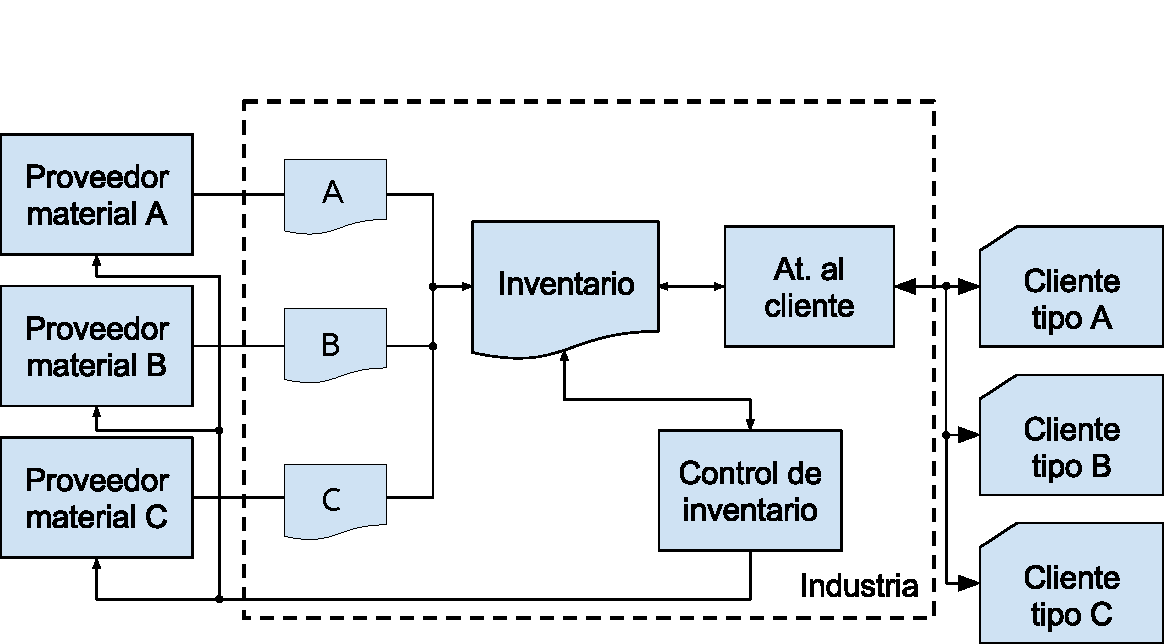
\includegraphics[width=\textwidth]{img/figura1}
\caption{Esquema del problema planteado.}
\label{fig:esquema-del-problema}
\end{figure}

La pregunta a responder mediante simulaciones es:
\textit{¿Qué política de reposición nos llevará a un manejo óptimo del nivel de stock logrando la mayor satisfacción del cliente y el menor costo de mantenimiento y reposición del inventario?}.

Una pregunta adicional que surge a partir de la anterior es:
\textit{¿Cómo ponderar adecuadamente ambos requisitos en conflicto?}
\FloatBarrier

\subsection{Descripción funcional}
A continuación se describen cada uno de los bloques de la Figura \ref{fig:esquema-del-problema}.

\subsubsection{Demanda (cliente)\label{sec:CLI}}
Los tiempos entre demandas por tipo de cliente son variables aleatorias exponenciales e independientemente distribuidas con una media de 0,12 mes. Los tamaños de las demandas (que pueden ir de uno a cuatro unidades del producto), D, son variables aleatorias independientemente distribuidas e independientes, cuya probabilidad de ocurrencia se muestra en la Tabla~\ref{tab:tabla1}.

\begin{table}[ht]
\begin{center}
\begin{tabular}{cc}
\toprule
\textbf{D (\# Unidades)} & \textbf{Probabilidad}\\
\midrule
1 unidad & $1/6$\\
2 unidades & $1/3$\\
3 unidades & $1/3$\\
4 unidades & $1/6$\\
\bottomrule
\end{tabular}
\end{center}
\caption{Demanda.}
\label{tab:tabla1}
\end{table}

Existen 3 tipos de políticas de demanda: A, B y C.
Un cliente tipo A encarga siempre $n$ productos y los retira a principio de mes. Un cliente tipo B pide $n$ productos pero se lleva solamente los que haya disponibles en stock en ese momento y los restantes para completar su pedido quedan encargados. Finalmente un cliente tipo C pide $n$ productos pero solamente compra si están disponibles, sino rechaza la compra.

El modelo que representa el comportamiento de los clientes tipo A se puede observar en la Figura~\ref{fig:fig2}, donde la salida \texttt{E\_OUT} indica la cantidad de productos encargados.

\begin{figure}[h]
\centering
\includegraphics[scale=1]{img/figura2}
\caption{Modelo de cliente tipo A.}
\label{fig:fig2}
\end{figure}

El modelo utilizado para el comportamiento de los clientes de tipo B se muestra en la Figura~\ref{fig:fig3}. Las salidas \texttt{P\_OUT}, \texttt{E\_OUT} y \texttt{Q\_OUT} indican respectivamente la cantidad de productos retirados, la cantidad de productos encargados y la cantidad de productos pedidos.

\begin{figure}[H]
\centering
\includegraphics[scale=1]{img/figura3}
\caption{Modelo de cliente tipo B.}
\label{fig:fig3}
\end{figure}

Finalmente, el modelo del comportamiento de los clientes de tipo C se muestra en la Figura~\ref{fig:fig4}.

\begin{figure}[h]
\centering
\includegraphics[scale=1]{img/figura4}
\caption{Modelo de cliente tipo C.}
\label{fig:fig4}
\end{figure}
\FloatBarrier

\subsubsection{Atención al cliente y control de calidad}
En la Figura~\ref{fig:fig5} se puede observar la interfaz del módulo de Atención al Cliente y Control de Calidad.
El departamento de Control de Calidad se encarga de examinar los productos al momento de venta y verificar su fecha de vencimiento. Los insumos con los que se elabora el producto son perecederos y la fecha de vencimiento del mismo se calcula con la fecha de vencimiento mínima de los insumos con los que se lo elaboró. La compañía descubre que una unidad no sirve más solamente cuando la examina debido a una venta. Si una unidad no sirve más, se desecha y se examina la siguiente unidad existente en el inventario.
El departamento de atención al cliente se encarga de realizar la negociación con los distintos tipos de clientes. Es decir, consulta al inventario la cantidad de productos disponibles al recibir una consulta del cliente y le informa dicho dato al mismo. También procesa el pedido de compra de cada cliente.
             
\begin{figure}[h]
\centering
\includegraphics[scale=0.8]{img/figura5}
\caption{Atención al cliente.}
\label{fig:fig5}
\end{figure}
\FloatBarrier

\subsubsection{Control de inventario\label{sec:CID}}

Al comienzo de cada mes, la compañía revisa el nivel de inventario y decide cuántas nuevas unidades pedir a sus proveedores. La compañía ordena $Z$ unidades a todos los proveedores por igual. El costo costo será $K + pZ$, donde $K = 350~\textrm{pesos}$ es el costo fijo del pedido y $p = 25~\textrm{pesos}$ es el costo incremental por unidad. Naturalmente, si $Z = 0$ no se incurre en ningún costo. La compañía usa la siguiente política para decidir cuántas unidades pedir: si $I$ es el nivel de inventario al comienzo del mes, $S$ el inventario máximo posible (capacidad de almacenamiento) y $n$ el parámetro de política de reposición, $Z$ estará dado por:

\begin{equation}
Z=\left\{\begin{array}{lr}
		S – I & \textrm{si}\qquad I < n\\
		0 & \textrm{si} \qquad I \geq n
	\end{array}\right.
\label{eq:ctrlinv}
\end{equation}

El modelo está dado por la Figura~\ref{fig:fig6}, donde se observa que hay tres estados: Query, Calc y Wait.

\begin{figure}[h]
\centering
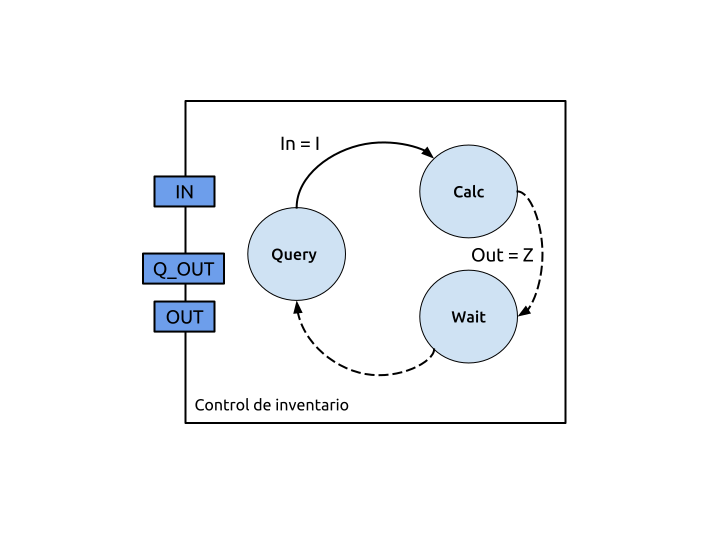
\includegraphics[scale=1]{img/figura6}
\caption{Esquema del control de inventario.}
\label{fig:fig6}
\end{figure}
\FloatBarrier

\subsubsection{Inventario}

Ante una consulta de un cliente el inventario responde con la cantidad de unidades disponibles en ese momento. En base a esto y a la política de cada cliente, al inventario se le pide una cantidad determinada de unidades para retiro y/ó encargue.
El inventario lleva una lista de unidades disponibles y una de unidades encargadas. Cuando una reposición llega, se usa primero para eliminar todos los pedidos pendientes (si hay) posibles; el resto de la reposición (si queda) se suma al inventario. 

\begin{figure}[h]
\centering
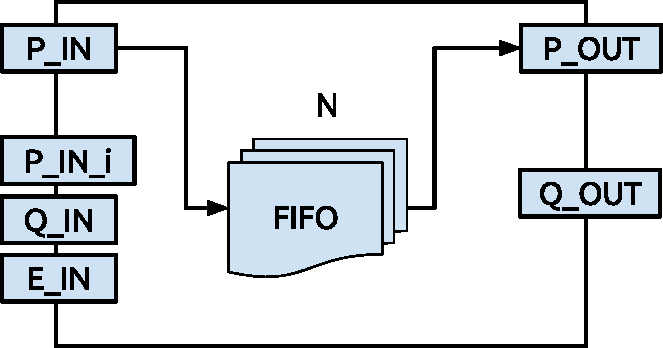
\includegraphics[scale=1]{img/figura7}
\caption{Inventario.}
\label{fig:fig7}
\end{figure}

En la Figura~\ref{fig:fig7} se observa el modelo con que se representa al Inventario. El mismo consiste de una cola FIFO (\textit{first in - first out}). Se denomina $N$ al largo de la cola.
Suponemos también que la compañía incurre en un costo de mantenimiento del producto $h = 8~\textrm{pesos}$ por unidad por mes mantenido en inventario (positivo). Este costo incluye alquiler del depósito de almacenamiento, seguro, impuestos y mantenimiento, al igual que costo de oportunidad de tener capital inmovilizado en inventario en vez de invertido en otra parte. Supongamos además que hay un costo de \textit{demanda insatisfecha} $n = 50~\textrm{pesos}$ por unidad pedida por cliente y no suministrada y por mes. Este costo contabiliza tanto el costo de mantener registros adicionales para unidades ya asignadas a clientes y aún no suministradas como un cálculo de costo por pérdida de la buena voluntad del cliente.
\FloatBarrier

\subsubsection{Proveedores}

Los proveedores se comportan de 3 formas diferentes: 
\begin{enumerate}[i)]
\item inmediato.
\item por múltiplo de cantidad fija.
\item por encargo.
\end{enumerate}

\begin{enumerate}[i)]
\item Al hacer un pedido al proveedor inmediato de $n$ unidades, entrega las $n$ unidades en forma instantánea. Las $n$ unidades asociadas tienen un tiempo de vencimiento asociado (Figura~\ref{fig:fig8}).

\begin{figure}
\centering
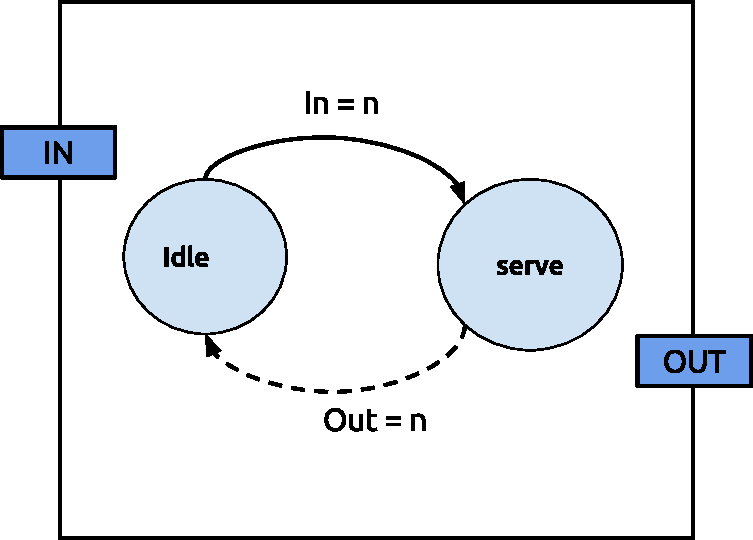
\includegraphics[scale=0.8]{img/figura8}
\caption{Proveedor Inmediato.}
\label{fig:fig8}
\end{figure}

\item El proveedor que funciona por múltiplo de cantidad fija, sólo entrega pedidos múltiplos de un número entero prefijado, digamos r (Figura~\ref{fig:fig9}). Es decir, que al hacer un pedido de n productos, pueden pasar 2 cosas:

\begin{enumerate}[1)]
\item El número pedido $n$ equivale a un múltiplo entero de $r$, $n = k r$, para algún $k \geq 0$, en cuyo caso se entregan exactamente $n$ unidades.
\item El número pedido $n$ es mayor a un múltiplo entero de $r$, es decir, $n > k r$ y además $n < (k+1)r$, para algún $k \geq 0$, en cuyo caso se entregan $(k+1)r$ unidades.
\end{enumerate}

Los productos de este proveedor no tienen vencimiento.

\begin{figure}
\centering
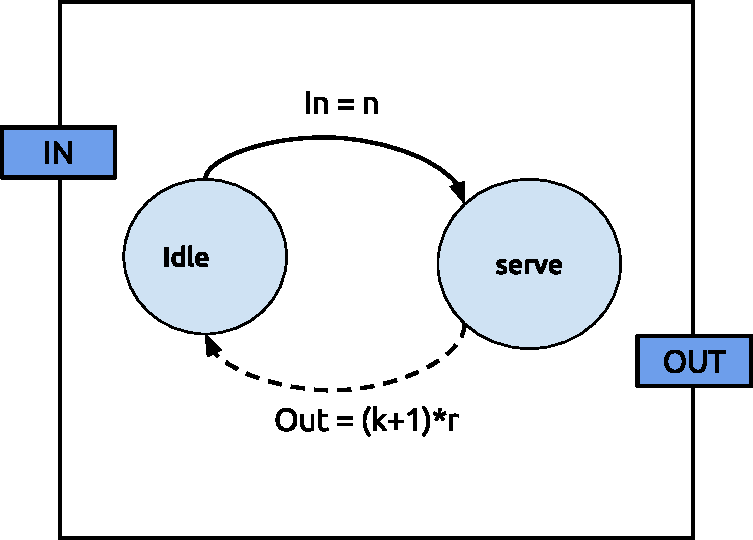
\includegraphics[scale=0.8]{img/figura9}
\caption{Proveedor por múltiplo de cantidad fija.}
\label{fig:fig9}
\end{figure}

\item El tercer proveedor (Figura~\ref{fig:fig10}) funciona por encargo para el mes siguiente. Es decir, todo pedido será servido en el siguiente mes. En ese momento, además, se realizará el nuevo pedido.

\begin{figure}
\centering
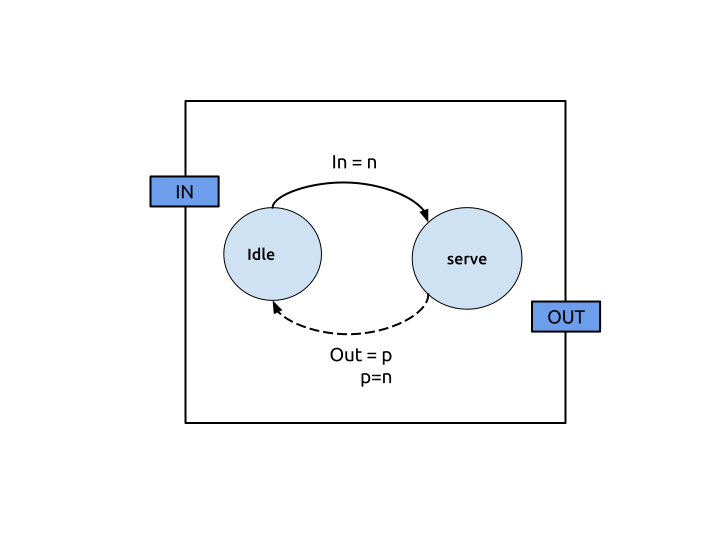
\includegraphics[scale=0.8]{img/figura10}
\caption{Proveedor por encargo.}
\label{fig:fig10}
\end{figure}
\end{enumerate}
\FloatBarrier

\section{Descripción Formal}

\subsection{\textit{Top Model}\label{sec:TM}} 
El diagrama de bloques correspondiente a cada uno de los atómicos descriptos en la especificación funcional se puede ver en la figura \ref{fig:TM-esquematico}.  
 
\begin{figure}[h] 
  \centering 
  \includegraphics[angle=-90, width=\textwidth]{img/bloquestopmodel} 
  \caption{Interconexión de bloques en el \texttt{top model}.} 
  \label{fig:TM-esquematico} 
\end{figure}
\FloatBarrier

\subsection{Tipo de Cliente A\label{sec:CTA}}

El modelo atómico correspondiente al bloque del cliente tipo A (CTA) queda definido de la siguiente manera:

\framebox[0.95\textwidth]{
	\begin{minipage}{0.9\textwidth}
		$CTA=<S,X,Y,\delta_{int},\delta_{ext},\lambda,t_A>$\\
		
		$S=\{QUERY \}$\\
		
		$X=\{\O \}$\\
		
		$Y=\{query\_o\}  \in \mathbb{N}^+_0$\\
		
		$\delta_{int}: \delta_{int}(QUERY)=QUERY$\\
		
		$\delta_{ext}:\emptyset$\\
		
		$\lambda:~\lambda(QUERY)=\{query\_o = N\}$\\
		
		$t_A(QUERY)=EXP\_VAR$
	\end{minipage}
}\\

En las figuras \ref{fig:CTA-esquematico} y \ref{fig:CTA-estados} se pueden observar los puertos de entrada/salida y el diagrama de estados respectivamente.

\begin{figure}[h]
	\centering
	\includegraphics{img/CTA-esquematico}
	\caption{Entradas y salidas del modelo del cliente tipo A.}
	\label{fig:CTA-esquematico}
\end{figure}

\begin{figure}[h] 
  \centering 
  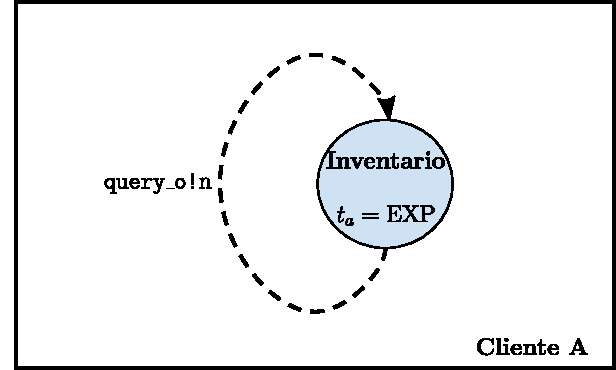
\includegraphics{img/clienteAdevsgraph} 
  \caption{Diagrama de estados para el modelo del cliente tipo A.} 
  \label{fig:CTA-estados} 
\end{figure} 
\FloatBarrier

\subsection{Tipo de Cliente B\label{sec:CTB}} 
El modelo atómico correspondiente al bloque del cliente tipo B (CTB) queda definido de la siguiente manera: 

\framebox[0.95\textwidth]{
	\begin{minipage}{0.9\textwidth}
		$CTB=<S,X,Y,\delta_{int},\delta_{ext},\lambda,t_A>$\\
		
		$S=\{IDLE, QUERY, CALC\}$\\
		
		$X=\{disponibles\_i \} \in \mathbb{N}^+_0$\\
		
		$Y=\{query\_o, pedido\_o\}  \in \mathbb{N}^+_0$\\
		
		$\delta_{int}: \delta_{int}(S) \begin{cases}
		\delta_{int}(IDLE)=QUERY\\
		\delta_{int}(CALC)=IDLE\\
		\end{cases}$\\
		
		$\delta_{ext}:\delta_{ext}(S,X) \begin{cases} Si ~S=QUERY \wedge  disponibles\_i=P\\
		\hfill \rightarrow \delta_{ext}(QUERY,disponibles\_i)=CALC\\
		\end{cases}$\\
		
		$\lambda:~\lambda(S)\begin{cases}
		\lambda(IDLE)=\{query\_o = N\}\\
		\lambda(CALC)=\{pedido\_o = P\}\\
		\end{cases}$\\
		
		$t_A(S)=\begin{cases}
		0~si~S=\{CALC\}\\
		\infty~si~S=\{QUERY\}\\
		EXP\_VAR~si~S=\{IDLE\}\
		\end{cases}$
	\end{minipage}
}\\

En las figuras \ref{fig:CTB-esquematico} y \ref{fig:CTB-estados} se pueden observar los puertos de entrada/salida y el diagrama de estados respectivamente.

\begin{figure}[h]
	\centering
	\includegraphics{img/CTB-esquematico}
	\caption{Entradas y salidas del modelo del cliente tipo B.}
	\label{fig:CTB-esquematico}
\end{figure}

\begin{figure}[h]
	\centering
	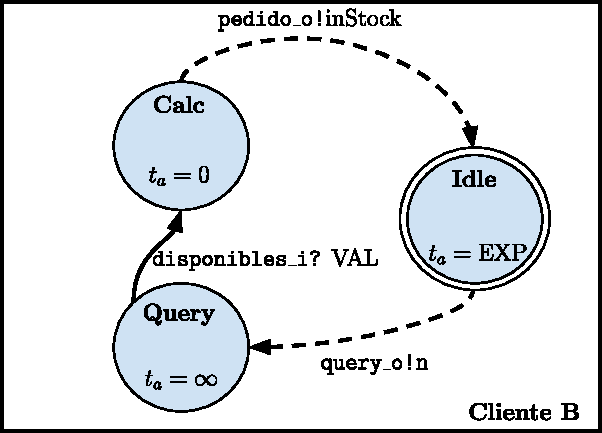
\includegraphics{img/clienteBdevsgraph}
	\caption{Diagrama de estados para el modelo del cliente tipo B.}
	\label{fig:CTB-estados}
\end{figure}
\FloatBarrier

\subsection{Tipo de Cliente C\label{sec:CTC}}

El modelo atómico correspondiente al bloque del cliente tipo C (CTC) queda definido de la siguiente manera:

\framebox[0.95\textwidth]{
	\begin{minipage}{0.9\textwidth}
		$CTC=<S,X,Y,\delta_{int},\delta_{ext},\lambda,t_A>$\\
		
		$S=\{IDLE, QUERY, ACCEPT, DECLINE\}$\\
		
		$X=\{disponibles\_i \} \in \mathbb{N}^+_0$\\
		
		$Y=\{query\_o, pedido\_o\}  \in \mathbb{N}^+_0$\\
		
		$\delta_{int}: \delta_{int}(S) \begin{cases}
		\delta_{int}(IDLE)=QUERY\\
		\delta_{int}(DECLINE)=IDLE\\
		\delta_{int}(ACCEPT)=IDLE
		\end{cases}$\\
		
		$\delta_{ext}:\delta_{ext}(S,X) \begin{cases} Si ~S=QUERY \wedge  disponibles\_i=N\\
		\hfill \rightarrow \delta_{ext}(QUERY,disponibles\_i)=ACCEPT\\
		Si ~S=QUERY \wedge disponibles\_i < N\\
		\hfill \rightarrow \delta_{ext}(QUERY,disponibles\_i)=DECLINE\\
		\end{cases}$\\
		
		$\lambda:~\lambda(S)\begin{cases}
		\lambda(IDLE)=\{query\_o = N\}\\
		\lambda(DECLINE)=\{pedido\_o = 0\}\\
		\lambda(ACCEPT)=\{pedido\_o = N\}
		\end{cases}$\\
		
		$t_A(S)=\begin{cases}
		0~si~S=\{ACCEPT, DECLINE\}\\
		\infty~si~S=\{QUERY\}\\
		EXP\_VAR~si~S=\{IDLE\}\
		\end{cases}$
	\end{minipage}
}\\

En las figuras \ref{fig:CTC-esquematico} y \ref{fig:CTC-estados} se pueden observar los puertos de entrada/salida y el diagrama de estados respectivamente.

\begin{figure}[h]
	\centering
	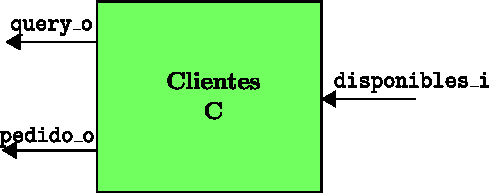
\includegraphics{img/CTC-esquematico}
	\caption{Entradas y salidas del modelo del cliente tipo C.}
	\label{fig:CTC-esquematico}
\end{figure}

\begin{figure}[h]
	\centering
	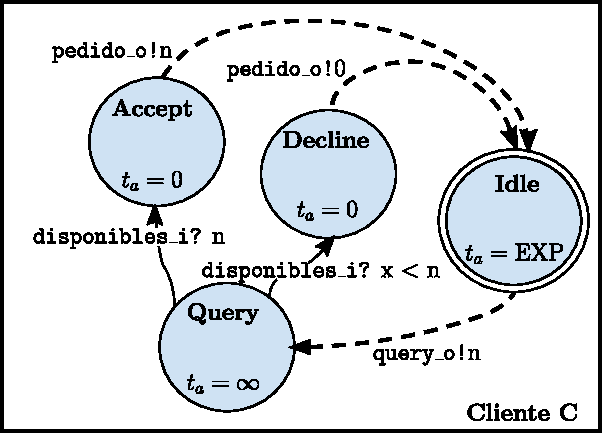
\includegraphics{img/clienteCdevsgraph}
	\caption{Diagrama de estados para el modelo del cliente tipo C.}
	\label{fig:CTC-estados}
\end{figure}
\FloatBarrier


\subsection{Control de inventario\label{sec:CI}}
El modelo atómico correspondiente al bloque de control de inventario (CI) queda definido de la siguiente manera:


\framebox[0.95\textwidth]{
\begin{minipage}{0.9\textwidth}
	$CI=<S,X,Y,\delta_{int},\delta_{ext},\lambda,t_A>$\\
	
	$S=\{WAITING, QUERY, CALC\}$\\
	
	$X=\{numProd\_i\} \in \mathbb{N}^+_0 $\\
	
	$Y=\{queryInventory\_o, querySuppliers\_o\} \in \mathbb{N}^+_0$\\
	
	$\delta_{int}: \delta_{int}(S) \begin{cases}
		\delta_{int}(WAITING)=QUERY\\
		\delta_{int}(CALC)=WAITING
		\end{cases}$\\
		
	$\delta_{ext}:\delta_{ext}(S,numProd\_i) \begin{cases} Si ~S=QUERY \wedge  numProd\_i=N\\
	\hfill \rightarrow \delta_{ext}(S,numProd\_i)=CALC \end{cases}$\\
	
	$\lambda:~\lambda(S)\begin{cases}
	\lambda(WAITING)=\{queryInventory\_o = 1\}\\
	\lambda(CALC)=\{ querySuppliers\_o = \begin{cases}
		S-N~si~numProd\_i\\
		\hfill < s\\
		0~\forall~numProd\_i
		\end{cases} \}
	\end{cases}$\\
	
	$t_A(S)=\begin{cases}
	1~si~S=WAITING\\
	0~si~S=CALC\\
	\infty~si~S=QUERY
	\end{cases}$
\end{minipage}
}

En las figuras \ref{fig:CI-esquematico} y \ref{fig:CI-estados} se pueden observar los puertos de entrada/salida y el diagrama de estados respectivamente.

\begin{figure}[h]
	\centering
	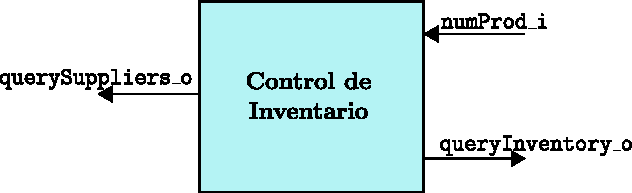
\includegraphics{img/CI-esquematico}
	\caption{Entradas y salidas del modelo control de inventario}
	\label{fig:CI-esquematico}
\end{figure}

\begin{figure}[h]
	\centering
	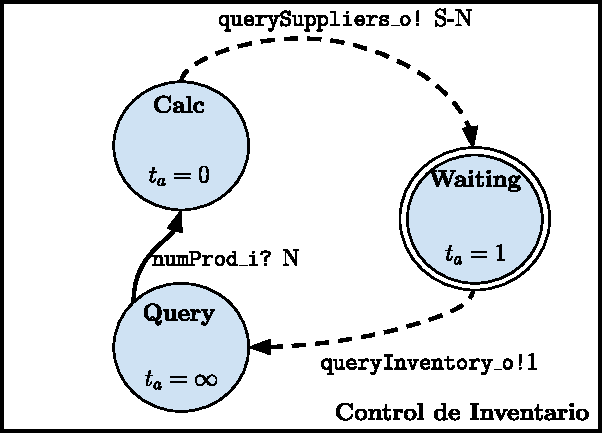
\includegraphics{img/controlInventariodevsgraph}
	\caption{Diagrama de estados para el modelo de control de inventario.}
	\label{fig:CI-estados}
\end{figure}
\FloatBarrier

\subsection{Control de Calidad\label{sec:CC}}
El modelo atómico correspondiente al bloque de control de calidad (CC) queda definido de la siguiente manera:

\framebox[0.95\textwidth]{
	\begin{minipage}{0.9\textwidth}
		$CC=<S,X,Y,\delta_{int},\delta_{ext},\lambda,t_A>$\\
		
		$S=\{WAITING, QUERY, INV\_WAIT, CHECK, SEND\}$\\
		
		$X=\{prod\_i \in \mathbb{R}^+, queryClient\_i \in \mathbb{N}^+_0 \}$\\
		
		$Y=\{prod\_o \in \mathbb{R}^+, queryInventory\_o  \in \mathbb{N}^+_0\}$\\
		
		$\delta_{int}: \delta_{int}(S) \begin{cases}
		\delta_{int}(QUERY)=INV\_WAIT\\
		\delta_{int}(CHECK)=\begin{cases}
		QUERY\\
		\hfill si~(numPassProd <\\
		\hfill numClientQuery)~\wedge\\
		\hfill (\neg{invEmpty})\\
		SEND~\forall~otra~condicion.
		\end{cases}\\
		\delta_{int}(SEND)=WAITING
		\end{cases}$\\
		
		$\delta_{ext}:\delta_{ext}(S,X) \begin{cases} Si ~S=WAITING \wedge  queryClient\_i=N\\
		\hfill \rightarrow \delta_{ext}(QUERY,queryClient\_i)=QUERY\\
		Si ~S=CHECK \wedge size(prod\_i)=P\\
		\hfill \rightarrow \delta_{ext}(CHECK,prod\_i)=SEND
		 \end{cases}$\\
		
		$\lambda:~\lambda(S)\begin{cases}
		\lambda(QUERY)=\{queryInventory\_o = 1\}\\
		\lambda(CHECK)=\{\O\}\\
		\lambda(SEND)=\{prod\_o = K\}
		\end{cases}$\\
		
		$t_A(S)=\begin{cases}
		0~si~S=\{QUERY,CHECK,SEND\}\\
		\infty~si~S=\{WAITING, INV\_WAIT\}
		\end{cases}$
	\end{minipage}
}\\

Donde:\\
$numPassProd = $ es el número de productos que pasan el control de calidad (i.e. su fecha de expiración es mayor al tiempo en que se produce el control).\\
$numClientQuery = $ es el número de productos que solicitó el cliente.\\
$invEmpty = $ es un Flag que indica si el inventario está vacío (i.e. devolvió un producto con fecha de expiración $0.0$)\footnote{el símbolo $\neg$ refiere a la condición lógica de negación}

En las figuras \ref{fig:CC-esquematico} y \ref{fig:CC-estados} se pueden observar los puertos de entrada/salida y el diagrama de estados respectivamente.

\begin{figure}[h]
	\centering
	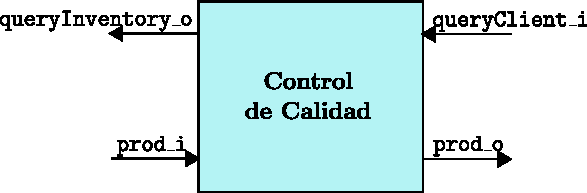
\includegraphics{img/CC-esquematico}
	\caption{Entradas y salidas del modelo control de calidad.}
	\label{fig:CC-esquematico}
\end{figure}

\begin{figure}[h]
	\centering
	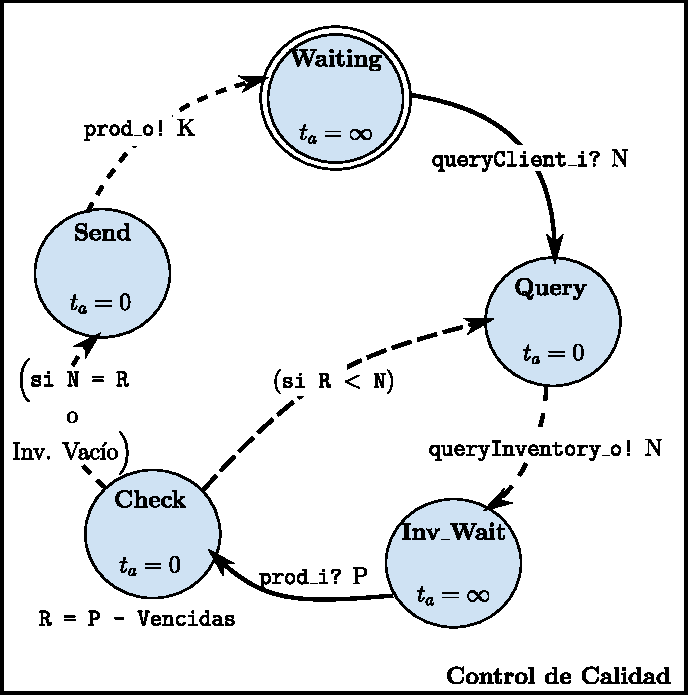
\includegraphics{img/controlCalidaddevsgraph}
	\caption{Diagrama de estados para el modelo de control de calidad.}
	\label{fig:CC-estados}
\end{figure}
\FloatBarrier

\subsection{Atención al cliente\label{sec:AC}}
El modelo atómico correspondiente al bloque de atención al cliente (AC) queda definido de la siguiente manera:

\framebox[0.95\textwidth]{
	\begin{minipage}{0.94\textwidth}%
		$AC=<S,X,Y,\delta_{int},\delta_{ext},\lambda,t_A>$\\
		
		$S=\{WAITING, QUERY, INV\_WAIT,\\
		\hfill CLI\_RPLY, CLI\_WAIT, INV\_GET\}$\\
		
		$X=\{numProdClient\_i, queryClient\_i, queryInventory\_i \} \in \mathbb{N}^+_0$\\
		
		$Y=\{prodInventory\_o, queryInventory\_o, queryClient_o\}  \in \mathbb{N}^+_0$\\
		
		$\delta_{int}: \delta_{int}(S) \begin{cases}
		\delta_{int}(QUERY)=INV\_WAIT\\
		\delta_{int}(CLI\_RPLY)=CLI\_WAIT\\
		\delta_{int}(INV\_GET)=WAITING
		\end{cases}$\\
		
		$\delta_{ext}:\delta_{ext}(S,X) \begin{cases} Si ~S=WAITING \wedge  queryClient\_i=N\\
		\hfill \rightarrow \delta_{ext}(WAITING,queryClient\_i)=QUERY\\
		Si ~S=INV\_WAIT \wedge queryInventory\_i=P\\
		\hfill \rightarrow \delta_{ext}(INV\_WAIT,queryInventory\_i)=CLI\_RPLY\\
		Si ~S=CLI\_WAIT \wedge numProdClient\_i=K\\
		\hfill \rightarrow \delta_{ext}(CLI\_WAIT,numProdClient\_i)=INV\_GET
		\end{cases}$\\
		
		$\lambda:~\lambda(S)\begin{cases}
		\lambda(QUERY)=\{queryInventory\_o = N\}\\
		\lambda(CLI\_RPLY)=\{queryCLient\_o = P\}\\
		\lambda(INV\_GET)=\{prodInventory\_o = K\}
		\end{cases}$\\
		
		$t_A(S)=\begin{cases}
		0~si~S=\{QUERY,CLI\_RPLY,INV\_GET\}\\
		\infty~si~S=\{WAITING, INV\_WAIT, CLI\_WAIT\}
		\end{cases}$
	\end{minipage}%
}\\

En las figuras \ref{fig:AC-esquematico} y \ref{fig:AC-estados} se pueden observar los puertos de entrada/salida y el diagrama de estados respectivamente.

\begin{figure}[h]
	\centering
	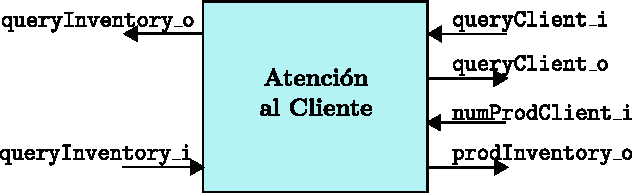
\includegraphics{img/AC-esquematico}
	\caption{Entradas y salidas del modelo atención al cliente.}
	\label{fig:AC-esquematico}
\end{figure}

\begin{figure}[h]
	\centering
	\includegraphics{img/atencionClientedevsgraph}
	\caption{Diagrama de estados para el modelo de atención al cliente.}
	\label{fig:AC-estados}
\end{figure}
\FloatBarrier

\subsection{Inventario\label{sec:I}}
El modelo atómico correspondiente al bloque de inventario (I) queda definido de la siguiente manera:

\framebox[0.95\textwidth]{
	\begin{minipage}{0.9\textwidth}
		$I=<S,X,Y,\delta_{int},\delta_{ext},\lambda,t_A>$\\
		
		$S=\{IDLE, QUERY, ENCARGO, PUSH, GET\}$\\
		
		$X=\{query\_in, encargo, producto\_in\_A,$\\
		\hfill $producto\_in\_B, producto\_in\_C, encargo, get \} \in \mathbb{N}^+_0$\\
		
		$Y=\{producto\_out, query\_out\}  \in \mathbb{N}^+_0$\\
		
		$\delta_{int}: \delta_{int}(S) \begin{cases}
		\delta_{int}(QUERY)=IDLE\\
		\delta_{int}(ENCARGO)=IDLE\\
		\delta_{int}(PUSH)=IDLE\\
		\delta_{it}(GET)=IDLE\\
		\end{cases}$\\
		
		$\delta_{ext}:\delta_{ext}(S,X) \begin{cases} Si ~S=IDLE \wedge \begin{cases} product\_in\_A = Na \\ product\_in\_B = Nb \\ product\_in\_C = Nc \\ \end{cases}\\
		\hfill \wedge ~size(cola\_i) == 0 ~\exists i \in \{A,B,C\}\\
		\hfill \rightarrow \delta_{ext}(IDLE,\{product\_in\_A, product\_in\_B \\
		\hfill product\_in\_C\})=QUERY\\
		Si ~S= IDLE \wedge encargo = Ne\\
		\hfill \rightarrow \delta_{ext}(IDLE,encargo)=ENCARGO\\
		Si ~S=IDLE \wedge \begin{cases} product\_in\_A = Na \\ product\_in\_B = Nb \\ product\_in\_C = Nc \\ \end{cases}\\
		\hfill \wedge ~size(cola\_i) != 0 ~\forall i \in \{A,B,C\}\\
		\hfill \rightarrow \delta_{ext}(IDLE,\{product\_in\_A, product\_in\_B \\
		\hfill product\_in\_C\})=PUSH\\
		Si ~S=IDLE \wedge get = Ng\\
		\hfill \rightarrow \delta_{ext}(IDLE,get)=GET
		\end{cases}$\\
		
		$\lambda:~\lambda(S)\begin{cases}
		\lambda(QUERY)=\{query\_out = size(cola) - encargos\_q\}\\
		\lambda(ENCARGO)=\{\O\}\\
		\lambda(PUSH)=\{producto\_out = \min(get\_q,size(cola))\}\\
		\lambda(GET)=\{producto\_out = \min(encargos\_q,size(cola))\}\\
		\end{cases}$\\
		
		$t_A(S)=\begin{cases}
		0~si~S=\{QUERY,ENCARGO,PUSH,GET\}\\
		\infty~si~S=\{IDLE\}
		\end{cases}$
	\end{minipage}
}\\

Donde:\\
$cola = $ es la cola de productos terminados.\\ 
$encargo\_q = $ es la cantidad de productos encargados por clientes que no estaban disponibles para entrega inmediata.\\
$get\_q = $ es la cantidad de productos pedidos después de consultar la cantidad de productos disponibles.\\

La negociación entre los estados IDLE y GET es una \textit{negociación segura}, es decir, se produce después de consultar al inventario la cantidad de productos disponibles. En caso que entre esta consulta y la compra ya no estén disponibles, porque en el medio se produjo una venta o porque alguno de los productos estaba vencido, se indica al control de calidad devolviendo un $0$. Esos productos indicados con $0$ no se reintegran a futuro.

En las figuras \ref{fig:I-esquematico} y \ref{fig:I-estados} se pueden observar los puertos de entrada/salida y el diagrama de estados respectivamente.

\begin{figure}[htbp]
	\centering
	\includegraphics{img/I-esquematico}
	\caption{Entradas y salidas del modelo inventario.}
	\label{fig:I-esquematico}
\end{figure}

\begin{figure}[htbp]
	\centering
	\includegraphics{img/Inventariodevsgraph}
	\caption{Diagrama de estados para el modelo de inventario.}
	\label{fig:I-estados}
\end{figure}
\FloatBarrier

\subsection{Industria}
La industria se instancia como un modelo acoplado definido de la siguiente manera:\\

\framebox[0.95\textwidth]{
	\begin{minipage}{0.9\textwidth}
		$IND=<X,Y, M_i, EIC, EOC, IC, Select>$\\
		
		$X=\{prod\_i\_A, prod\_i\_B, prod\_i\_C, queryClient\_i,\\
		\hfill encargo\_i, numProdClient\_i\}\in \mathbb{N}^+_0$\\
		
		$Y=\{prod\_o\} \in \mathbb{R}^+ 
		\bigcup \; \{queryClient\_o, querySuppliers\_o\}\in \mathbb{N}^+_0 $\\
		
		$M=\{I, CI, CC, AC\}$\\
		
		$EIC=\{(prod\_i\_A, I.products\_in\_A), (prod\_i\_B,  I.products\_in\_B),\\
		(prod\_i\_C, I.products\_in\_C), (queryClient\_i,AC.queryClient\_i),\\
		\hfill (encargo\_i,I.encargo), (numProdClient\_i, AC.numProdClient\_i)\}$\\
		
		$IC=\{(AC.queryInventory\_o,I.query\_i),\\ (AC.queryInventory\_i,I.query\_out),\\
		(CI.queryInventory\_o,I.query\_i),  (CI.numProd\_i,I.query\_out)\\
		(CC.prod\_i,I.product\_o), (CC.queryInventory\_o,I.get),\\
		(AC.prodInventory_o, queryClient_i)
		\}$\\
		
		$EOC=\{(prod\_o,CC.prod_o),(queryClient\_o,CI.prod\_o),\\
		\hfill (querySuppliers\_o,)\}$\\
		
		$Select=\{\{I,CI,AC,CC\} = CI\\
		\{I,AC,CC\} = I\\
		\{AC,CC\} = AC\}$
	\end{minipage}
}\\

\subsection{Proveedor Inmediato\label{sec:PI}}
El modelo atómico correspondiente al bloque del proveedor inmediato (PI) queda definido de la siguiente manera:

\framebox[1\textwidth]{
	\begin{minipage}{0.9\textwidth}
		$PI=<S,X,Y,\delta_{int},\delta_{ext},\lambda,t_A>$\\
		
		$S=\{IDLE, SERVE\}$\\
		
		$X=\{pedido \} \in \mathbb{N}^+_0$\\
		
		$Y=\{entrega \}  \in \mathbb{N}^+_0$\\
		
		$\delta_{int}: \delta_{int}(SERVE) = IDLE$\\
		
		$\delta_{ext}:\delta_{ext}(S,X) \begin{cases} Si ~S=IDLE \wedge  pedido = N\\
		\hfill \rightarrow \delta_{ext}(IDLE, pedido)=SERVE\\
		\end{cases}$\\
		
		$\lambda:~\lambda(SERVE)=\{entrega = N\}$\\
		
		$t_A(S)=\begin{cases}
		0~si~S=\{SERVE \}\\
		\infty~si~S=\{IDLE \}
		\end{cases}$
	\end{minipage}
}\\

En las figuras \ref{fig:PI-esquematico} y \ref{fig:PI-estados} se pueden observar los puertos de entrada/salida y el diagrama de estados respectivamente.

\begin{figure}[htbp]
	\centering
	\includegraphics{img/PI-esquematico}
	\caption{Entradas y salidas del modelo del proveedor inmediato}
	\label{fig:PI-esquematico}
\end{figure}

\begin{figure}[htbp]
	\centering
	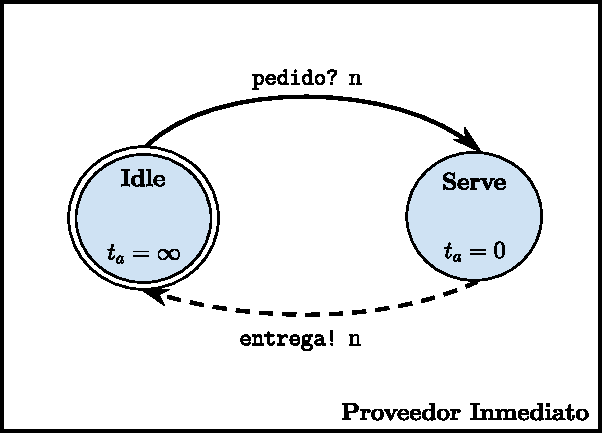
\includegraphics{img/proveedorInmediatodevsgraph}
	\caption{Diagrama de estados para el modelo del proveedor inmediato.}
	\label{fig:PI-estados}
\end{figure}
\FloatBarrier

\subsection{Proveedor por múltiplo de cantidad fija\label{sec:PF}}
El modelo atómico correspondiente al bloque del proveedor por múltiplo de cantidad fija (PF) queda definido de la siguiente manera:

\framebox[1\textwidth]{
	\begin{minipage}{0.9\textwidth}
		$PF=<S,X,Y,\delta_{int},\delta_{ext},\lambda,t_A>$\\
		
		$S=\{IDLE, SERVE\}$\\
		
		$X=\{pedido \} \in \mathbb{N}^+_0$\\
		
		$Y=\{entrega \}  \in \mathbb{N}^+_0$\\
		
		$\delta_{int}: \delta_{int}(SERVE) = IDLE$\\
		
		$\delta_{ext}:\delta_{ext}(S,X) \begin{cases} Si ~S=IDLE \wedge  pedido = N\\
		\hfill \rightarrow \delta_{ext}(IDLE, pedido)=SERVE\\
		\end{cases}$\\
		
		$\lambda:~\lambda(SERVE) = \{ entrega = \begin{cases}
		N~Si~N\%numProdPkg=0 \\
		\lfloor N/numProdPkg \rfloor \\
		\hfill + N\%numProdpkg~\forall~N
		\end{cases}$\}\\

		$t_A(S)=\begin{cases}
		0~si~S=\{SERVE \}\\
		\infty~si~S=\{IDLE \}
		\end{cases}$
	\end{minipage}
}\\

Donde:\\
$numProdPkg = $ es el número de productos por paquete cerrado que comercializa este proveedor.\\

En las figuras \ref{fig:PF-esquematico} y \ref{fig:PF-estados} se pueden observar los puertos de entrada/salida y el diagrama de estados respectivamente.

\begin{figure}[htbp]
	\centering
	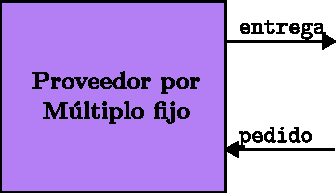
\includegraphics{img/PF-esquematico}
	\caption{Entradas y salidas del modelo del proveedor por múltiplo de cantidad fija}
	\label{fig:PF-esquematico}
\end{figure}

\begin{figure}[htbp]
	\centering
	\includegraphics{img/proveedorFijodevsgraph}
	\caption{Diagrama de estados para el modelo del proveedor por múltiplo de cantidad fija.}
	\label{fig:PF-estados}
\end{figure}
\FloatBarrier

\subsection{Proveedor por Encargo\label{sec:PE}}
El modelo atómico correspondiente al bloque del proveedor por encargo (PE) queda definido de la siguiente manera:

\framebox[1\textwidth]{
	\begin{minipage}{0.9\textwidth}
		$PE=<S,X,Y,\delta_{int},\delta_{ext},\lambda,t_A>$\\
		
		$S=\{IDLE, SERVE\}$\\
		
		$X=\{pedido \} \in \mathbb{N}^+_0$\\
		
		$Y=\{entrega \}  \in \mathbb{N}^+_0$\\
		
		$\delta_{int}: \delta_{int}(SERVE) = IDLE$\\
		
		$\delta_{ext}:\delta_{ext}(S,X) \begin{cases} Si ~S=IDLE \wedge  pedido = N\\
		\hfill \rightarrow \delta_{ext}(IDLE, pedido)=SERVE\\
		\end{cases}$\\
		
		$\lambda:~\lambda(SERVE)=\{entrega = N\}$\\
		
		$t_A(S)=\begin{cases}
		1~si~S=\{SERVE \}\\
		\infty~si~S=\{IDLE \}
		\end{cases}$
	\end{minipage}
}\\

En las figuras \ref{fig:PE-esquematico} y \ref{fig:PE-estados} se pueden observar los puertos de entrada/salida y el diagrama de estados respectivamente.

\begin{figure}[htbp]
	\centering
	\includegraphics{img/PE-esquematico}
	\caption{Entradas y salidas del modelo del proveedor por encargo}
	\label{fig:PE-esquematico}
\end{figure}

\begin{figure}[htbp]
	\centering
	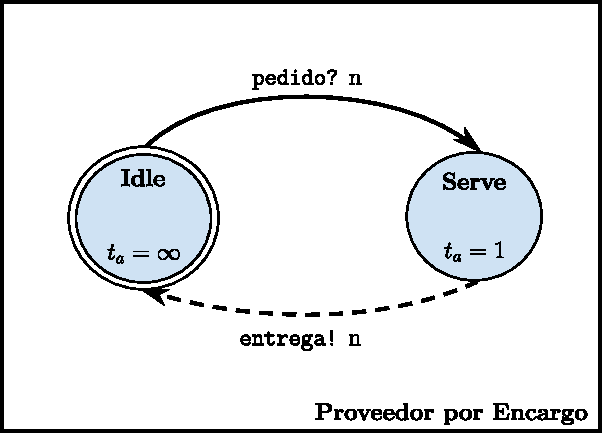
\includegraphics{img/proveedorEncargodevsgraph}
	\caption{Diagrama de estados para el modelo del proveedor por encargo.}
	\label{fig:PE-estados}
\end{figure}
\FloatBarrier

%%%%%%%%%%%%%%%%%%%%%%%%%%%%%%%%%%%%%%%%%%%%%%%%%%%%%%%%%%%%%%%%%%%%%%%%%%
\section{Modelado y simulación}
%%%%%%%%%%%%%%%%%%%%%%%%%%%%%%%%%%%%%%%%%%%%%%%%%%%%%%%%%%%%%%%%%%%%%%%%%%

\subsection{Pruebas parciales\label{sec:PP}}


 
\subsubsection{Demandas de los Clientes} 
 
En la Figura~\ref{fig:pdftiempo} y Figura~\ref{fig:pdfpedidos} se observan los histogramas que representan la tasa de arribos de pedidos de clientes y la cantidad de unidades pedidas. Se puede notar que la distribución de los tiempos de arribos sigue una distribución de probabilidad exponencial y el valor medio del tiempo entre arribos es de alrededor de $0.12$. La distribución de probbilidad de la cantidad de unidades pedidas corresponde a la mencionada en la sección \ref{sec:CLI}. 

En ambas figuras el tiempo se mide en segundos, aunque cada segundo representa un mes. 
 
\begin{figure} 
\centering 
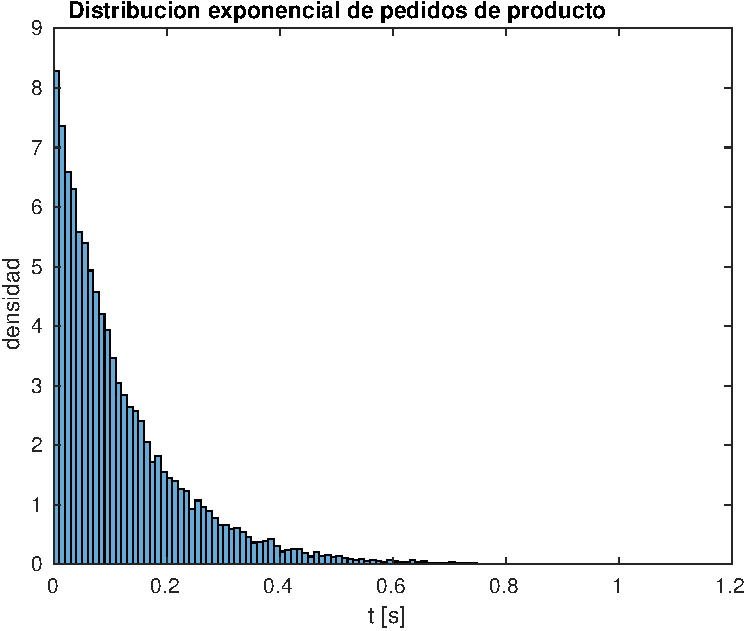
\includegraphics[width=0.6\textwidth]{img/pdf_tiempo_pedidos} 
\caption{Función de densidad de probabilidad del tiempo entre pedidos de clientes.} 
\label{fig:pdftiempo} 
\end{figure} 
 
\begin{figure} 
\centering 
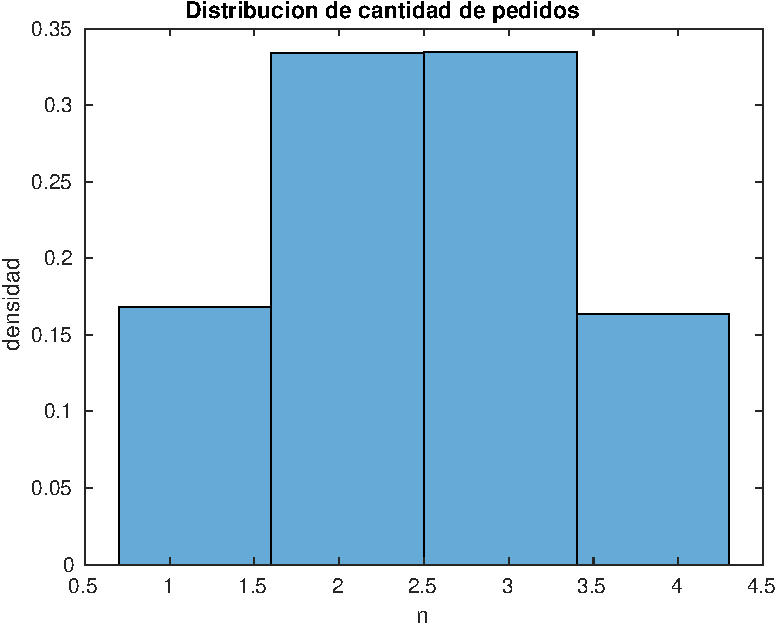
\includegraphics[width=0.6\textwidth]{img/pdf_cantidad_pedidos} 
\caption{Función de densidad de probabilidad del número de unidades pedidas $n$.} 
\label{fig:pdfpedidos} 
\end{figure}
\FloatBarrier

\subsubsection{Cliente A}
Para la prueba del bloque de clientes tipo A no se necesitan eventos de entrada porque este tipo de cliente encarga productos sin importar si están disponibles. La salida de la prueba es la siguiente:

\begin{minipage}{1\textwidth}
	\centering
	\begin{lstlisting}
00:00:00:073:0.401741 Client A - encargo: 1
00:00:00:101:0.768183 Client A - encargo: 4
00:00:00:322:0.663614 Client A - encargo: 4
00:00:00:385:0.395575 Client A - encargo: 2
00:00:00:585:0.052725 Client A - encargo: 2
00:00:00:604:0.393726 Client A - encargo: 3
	\end{lstlisting}
	
\end{minipage}
Con trazas como ésta se obtuvieron la Figura~\ref{fig:pdftiempo} y Figura~\ref{fig:pdfpedidos}. 

\subsubsection{Cliente B}
Para la prueba del bloque de clientes tipo B se propuso el siguiente estímulo:

\begin{minipage}{1\textwidth}
	\centering
	\begin{lstlisting}
00:00:05:00 in_port 1
00:00:30:00 in_port 0
00:00:45:00 in_port 10
00:01:20:00 in_port 1
	\end{lstlisting}
\end{minipage}

Dada la política de pedidos, se busca probar las condiciones:
\begin{itemize}
\item La cantidad de productos disponibles en el inventario es menor al valor consultado por el cliente, por lo tanto se piden las unidades disponibles y se encargan las restantes.
\item La cantidad de productos en el inventario es mayor o igual al valor consultado por el cliente, por lo tanto piden todas las unidades por las que se consultó.
\end{itemize}

La salida de la prueba es la siguiente:

\begin{minipage}{1\textwidth}
	\centering
	\begin{lstlisting}
00:00:00:073:0.401741 Client B - pregunta por: 1 productos
00:00:05:000:0 Client B - le dicen que hay: 1 productos
00:00:05:000:0 Client B - pide: 1
00:00:05:119:0.451668 Client B - pregunta por: 4 productos
00:00:30:000:0 Client B - le dicen que hay: 0 productos
00:00:30:000:0 Client B - pide: 0
00:00:30:000:0 Client B - encarga: 4
00:00:30:009:0.329481 Client B - pregunta por: 4 productos
00:00:45:000:0 Client B - le dicen que hay: 10 productos
00:00:45:000:0 Client B - pide: 4
00:00:45:003:0.96502 Client B - pregunta por: 2 productos
00:01:20:000:0 Client B - le dicen que hay: 1 productos
00:01:20:000:0 Client B - pide: 1
00:01:20:000:0 Client B - encarga: 1
	\end{lstlisting}
	
\end{minipage}
Donde se observa que se cumplen las condiciones mencionadas en la sección \ref{sec:CTB}, ya que si el número de unidades disponibles para entrega inmediata es menor a la cantidad consultada la compra se realiza igual.

\subsubsection{Cliente C}
Para la prueba del bloque de clientes de tipo C se propuso el siguiente estímulo:

\begin{minipage}{1\textwidth}
	\centering
	\begin{lstlisting}
00:00:05:00 in_port 1
00:00:30:00 in_port 0
00:00:45:00 in_port 10
00:01:20:00 in_port 1
	\end{lstlisting}
\end{minipage}

Dada la política de pedidos, se busca probar las condiciones:
\begin{itemize}
\item La cantidad de productos disponibles en el inventario es menor al valor consultado por el cliente, por lo tanto se rechaza la compra.
\item La cantidad de productos en el inventario es mayor o igual al valor consultado por el cliente, por lo tanto piden todas las unidades por las que se consultó.
\end{itemize}

La salida de la prueba es la siguiente:

\begin{minipage}{1\textwidth}
	\centering
	\begin{lstlisting}
00:00:00:073:0.401741 Client C - pregunta por: 1 productos
00:00:05:000:0 Client C - Peticion aceptada
00:00:05:000:0 Client C - pide: 1 productos
00:00:05:119:0.451668 Client C - pregunta por: 4 productos
00:00:30:000:0 Client C - Peticion rechazada
00:00:30:000:0 Client C - No pide nada
00:00:30:009:0.329481 Client C - pregunta por: 4 productos
00:00:45:000:0 Client C - Peticion aceptada
00:00:45:000:0 Client C - pide: 4 productos
00:00:45:003:0.96502 Client C - pregunta por: 2 productos
00:01:20:000:0 Client C - Peticion rechazada
00:01:20:000:0 Client C - No pide nada
	\end{lstlisting}
	
\end{minipage}

Donde se observa que se cumplen las condiciones mencionadas en la sección \ref{sec:CTC}, ya que si el número de unidades disponibles para entrega inmediata es menor a la cantidad consultada entonces la compra no se realiza.

\subsubsection{Control de Inventario}
Para la prueba del bloque de control de inventario se propuso el siguiente estímulo:

\begin{minipage}{1\textwidth}
	\centering
	\begin{lstlisting}
00:00:01:10 numProd_i 8
00:00:02:10 numProd_i 190
00:00:03:10 numProd_i 49
	\end{lstlisting}
\end{minipage}

Dada la política de pedidos, se busca probar las condiciones:
\begin{itemize}
\item La cantidad de productos en el inventario es menor al valor requerido por la política de reposición, por lo tanto se debe pedir materiales a los proveedores.
\item  La cantidad de productos en el inventario es menor al máximo pero no alcanza el mínimo de la política de reposición por lo que no se deben pedir materiales.
\end{itemize}

La salida de la prueba es la siguiente:

\begin{minipage}{1\textwidth}
	\centering
	\begin{lstlisting}
00:00:01:000:0 Control Inventario - Consulta a Inventario
00:00:01:010:0 Control Inventario - Inventario responde: 8
00:00:01:010:0 Control Inventario - Pedido a proveedores: 92
00:00:02:010:0 Control Inventario - Consulta a Inventario
00:00:02:010:0 Control Inventario - Inventario responde: 190
00:00:02:010:0 Control Inventario - Pedido a proveedores: 0
00:00:03:010:0 Control Inventario - Consulta a Inventario
00:00:03:010:0 Control Inventario - Inventario responde: 49
00:00:03:010:0 Control Inventario - Pedido a proveedores: 51
00:00:04:010:0 Control Inventario - Consulta a Inventario
	\end{lstlisting}
	
\end{minipage}
Donde se observa que se cumplen las condiciones mencionadas en la sección \ref{sec:CI}, ya que si el número de unidades se encuentra por debajo del umbral de política, el bloque pide, y de lo contrario no. 

\subsubsection{Control de Calidad}
Para la prueba del bloque de control de calidad se propuso el siguiente estímulo:

\begin{minipage}{1\textwidth}
	\centering
	\begin{lstlisting}
00:00:01:00 queryClient_i 2
00:00:01:10 prod_i [1.2,1.3]
00:00:02:00 queryClient_i 3
00:00:02:10 prod_i [1.5,2.2,2.3]
00:00:02:20 prod_i [2.3]
00:00:03:00 queryClient_i 3
00:00:03:10 prod_i [3.2,3.3,0]
	\end{lstlisting}
\end{minipage}

Se busca probar las condiciones:
\begin{itemize}
	\item Un cliente compra $N$ productos y el inventario devuelve $N$ productos correctos. Por lo tanto se deberían enviar todos.
	\item Un cliente compra $N$ productos y el inventario devuelve $N-1$ productos correctos y uno vencido. Se debe descartar ese producto y pedir uno nuevo al inventario. El inventario devuelve un producto válido. Se deberían enviar los $N$ productos válidos.
	\item Un cliente compra N productos pero el inventario dispone sólo de $N-1$ y devuelve $0$ en la última posición. El control de calidad debe interpretar la salida y despachar sólo los dos productos correctos.
\end{itemize}

La salida de la prueba es la siguiente:

\begin{minipage}{1\textwidth}
	\centering
	\begin{lstlisting}
00:00:01:000:0 Control Calidad - le piden: 2 productos
00:00:01:000:0 Control Calidad - pide: 2 productos
00:00:01:010:0 Control Calidad - recibe 2 productos
00:00:01:010:0 Control Calidad - se queda con 2 productos
00:00:01:010:0 Control Calidad - envia: 2 productos
00:00:02:000:0 Control Calidad - le piden: 3 productos
00:00:02:000:0 Control Calidad - pide: 3 productos
00:00:02:010:0 Control Calidad - recibe 3 productos
00:00:02:010:0 Control Calidad - se queda con 2 productos
00:00:02:010:0 Control Calidad - pide: 1 productos
00:00:02:020:0 Control Calidad - recibe 1 productos
00:00:02:020:0 Control Calidad - se queda con 3 productos
00:00:02:020:0 Control Calidad - envia: 3 productos
00:00:03:000:0 Control Calidad - le piden: 3 productos
00:00:03:000:0 Control Calidad - pide: 3 productos
00:00:03:010:0 Control Calidad - recibe 3 productos
00:00:03:010:0 Control Calidad - se queda con 2 productos
00:00:03:010:0 Control Calidad - el inventario esta vacio
00:00:03:010:0 Control Calidad - envia: 2 productos
	\end{lstlisting}
	
\end{minipage}
Donde se observa que se cumplen las condiciones mencionadas en la sección \ref{sec:CC}.

\subsubsection{Atención al cliente}
Para la prueba del bloque de atención al cliente se propuso el siguiente estímulo:

\begin{minipage}{1\textwidth}
	\centering
	\begin{lstlisting}
00:00:01:00	queryClient_i 1
00:00:01:10 queryInventory_i 2
00:00:01:15 numProdClient_i 1
00:00:02:00	queryClient_i 3
00:00:02:10 queryInventory_i 2
00:00:02:15 numProdClient_i 2
00:00:03:00	queryClient_i 3
00:00:03:10 queryInventory_i 2
00:00:03:15 numProdClient_i 0
	\end{lstlisting}
\end{minipage}

Se busca probar las condiciones:
\begin{itemize}
	\item Un cliente solicita $N$ productos y el inventario devuelve una cantidad $> N$ que se le informa al cliente. Por lo tanto el cliente compra N productos.
	\item Un cliente solicita $N$ productos. El inventario responde con $P < N$ y el cliente decide comprar $P$ productos.
	\item Un cliente solicita $N$ productos. El inventario responde con $P < N$ y el cliente decide no comprar ningún producto.
\end{itemize}

La salida de la prueba es la siguiente:

\begin{minipage}{1\textwidth}
	\centering
	\begin{lstlisting}
00:00:01:000:0 Atencion al cliente - le piden 1 productos
00:00:01:000:0 Atencion al cliente - pregunta por 1 productos
00:00:01:010:0 Atencion al cliente - le dicen que hay 2 stock
00:00:01:010:0 Atencion al cliente - informa a cliente que hay 2 stock
00:00:01:015:0 Atencion al cliente - cliente pide 1 productos
00:00:01:015:0 Atencion al cliente - pide al inventario 1 productos
00:00:02:000:0 Atencion al cliente - le piden 3 productos
00:00:02:000:0 Atencion al cliente - pregunta por 3 productos
00:00:02:010:0 Atencion al cliente - le dicen que hay 2 stock
00:00:02:010:0 Atencion al cliente - informa a cliente que hay 2 stock
00:00:02:015:0 Atencion al cliente - cliente pide 2 productos
00:00:02:015:0 Atencion al cliente - pide al inventario 2 productos
00:00:03:000:0 Atencion al cliente - le piden 3 productos
00:00:03:000:0 Atencion al cliente - pregunta por 3 productos
00:00:03:010:0 Atencion al cliente - le dicen que hay 2 stock
00:00:03:010:0 Atencion al cliente - informa a cliente que hay 2 stock
00:00:03:015:0 Atencion al cliente - cliente pide 0 productos

	\end{lstlisting}
	
\end{minipage}
Donde se observa que se cumplen las condiciones mencionadas en la sección \ref{sec:AC}

\subsubsection{Inventario}
Para la prueba del bloque de inventario se propuso el siguiente estímulo:

\begin{minipage}{1\textwidth}
	\centering
	\begin{lstlisting}
00:00:05:00 query_in 1
00:00:09:00 producto_in_A [1.5,1.2,0.9]
00:00:51:00 producto_in_B [0.9,0.9,0.9]
00:00:54:00 query_in 1
00:00:55:00 producto_in_C [0.9,0.9,0.9]
00:00:58:00 query_in 1
00:00:59:00 get 2
00:00:60:00 encargo 1
00:00:61:00 query_in 1
00:00:62:00 producto_in_C [0.9,0.9,0.9]
00:00:63:00 producto_in_A [1.5,1.2,0.9]
00:00:64:00 producto_in_B [0.9,0.9,0.9]
00:00:65:00 query_in 1
00:00:66:00 get 2
00:00:67:00 get 2
	\end{lstlisting}
\end{minipage}

Se busca probar las condiciones:
\begin{itemize}
	\item Un proveedor entrega unidades de un insumo. El inventario lo almacena en la cola de insumo correspondiente. Cuando haya unidades de todos los insumos se obtendrán productos automáticamente.
	\item Un cliente encarga $Ne$ productos. El inventario incrementa la cantidad de unidades encargadas $E$.
	\item Un cliente consulta la disponibilidad de $Nq$ productos. El inventario responde con $N-E$, siendo $N$ la cantidad de productos disponibles y $E$ la cantidad de productos previamente encargados.
	\item Un cliente consulta la disponibilidad de $Nq$ productos. El inventario responde con $N \geq Nq$ y el cliente compra $M > Nq$, si están disponibles se le entregan las $M$ unidades y sino se le entregan $Nq$. 
\end{itemize}

La salida de la prueba es la siguiente:

\begin{minipage}{1\textwidth}
	\centering
	\begin{lstlisting}
00:00:05:000:0 Inventario - Query out(N - E): 0
00:00:05:000:0 Inventario - Cola(N): 0
00:00:54:000:0 Inventario - Query out(N - E): 0
00:00:54:000:0 Inventario - Cola(N): 0
00:00:55:000:0 Inventario - Entran 3 productos
00:00:55:000:0 Inventario - Hay en cola N:3
INVENTARIO , 00:00:55:000:0 , 3 , 0 , 0 , 0 , 0
00:00:58:000:0 Inventario - Query out(N - E): 3
00:00:58:000:0 Inventario - Cola(N): 3
00:00:59:000:0 Inventario - Entrega: [0.9, 0.9]
INVENTARIO , 00:00:59:000:0 , 1 , 0 , 0 , 0 , 0
00:01:00:000:0 Inventario - Encargos(E): 1
INVENTARIO , 00:01:00:000:0 , 1 , 0 , 0 , 0 , 1
00:01:01:000:0 Inventario - Query out(N - E): 0
00:01:01:000:0 Inventario - Cola(N): 1
00:01:04:000:0 Inventario - Entran 3 productos
00:01:04:000:0 Inventario - Encargos entregados:1
00:01:04:000:0 Inventario - Encargos restantes:0
00:01:04:000:0 Inventario - Hay en cola N:3
INVENTARIO , 00:01:04:000:0 , 3 , 0 , 0 , 0 , 0
00:01:05:000:0 Inventario - Query out(N - E): 3
00:01:05:000:0 Inventario - Cola(N): 3
00:01:06:000:0 Inventario - Entrega: [0.9, 0.9]
INVENTARIO , 00:01:06:000:0 , 1 , 0 , 0 , 0 , 0
00:01:07:000:0 Inventario - Entrega: [0.9, 0]
INVENTARIO , 00:01:07:000:0 , 0 , 0 , 0 , 0 , 0
	\end{lstlisting}
	
\end{minipage}
Donde se observa que se cumplen las condiciones mencionadas en la sección \ref{sec:I}. Se puede notar que hasta que no haya disponibles unidades de los insumos A, B y C no se pueden producir productos y que en caso contrario se producen instantáneamente.
Se puede notar que cuando se solicita una cantidad de productos mayor a la que se había consultado previamente se entregan unidades con fecha de vencimiento $0$, que representan que ese producto no está disponible al momento de la compra y no se va a encargar.


\subsubsection{Proveedor Inmediato}
Para la prueba del bloque proveedor inmediato se propuso el siguiente estímulo:

\begin{minipage}{1\textwidth}
	\centering
	\begin{lstlisting}
00:00:05:00 pedido 1 
00:00:09:00 pedido 4
00:00:17:00 pedido 3
00:00:50:00 pedido 2
	\end{lstlisting}
\end{minipage}

Se busca probar las condiciones:
\begin{itemize}
	\item El control de inventario solicita $N$ unidades de insumo y el proveedor responde instantáneamente. 
\end{itemize}

La salida de la prueba es la siguiente:

\begin{minipage}{1\textwidth}
	\centering
	\begin{lstlisting}
00:00:05:000:0 Proveedor Inmediato - Pedido: 1 productos
00:00:05:000:0 Proveedor Inmediato - Entrega: 1 productos
00:00:09:000:0 Proveedor Inmediato - Pedido: 4 productos
00:00:09:000:0 Proveedor Inmediato - Entrega: 4 productos
00:00:17:000:0 Proveedor Inmediato - Pedido: 3 productos
00:00:17:000:0 Proveedor Inmediato - Entrega: 3 productos
00:00:50:000:0 Proveedor Inmediato - Pedido: 2 productos
00:00:50:000:0 Proveedor Inmediato - Entrega: 2 productos
	\end{lstlisting}
	
\end{minipage}

Donde se observa que se cumplen las condiciones mencionadas en la sección \ref{sec:PI}.

\subsubsection{Proveedor por Múltiplo Fijo}
Para la prueba del bloque proveedor por múltiplo fijo se propuso el siguiente estímulo:

\begin{minipage}{1\textwidth}
	\centering
	\begin{lstlisting}
00:00:05:00 pedido 100
00:00:09:00 pedido 40
00:00:17:00 pedido 30
00:00:50:00 pedido 200
	\end{lstlisting}
\end{minipage}

Se busca probar las condiciones:
\begin{itemize}
	\item El control de inventario solicita $N$ unidades de insumo. El proveedor entrega instantáneamente con una cantidad múltiplo del número de unidades por paquete. 
\end{itemize}

La salida de la prueba es la siguiente:

\begin{minipage}{1\textwidth}
	\centering
	\begin{lstlisting}
00:00:05:000:0 Proveedor Fijo - Pedido: 100 productos
00:00:05:000:0 Proveedor Fijo - Entrega: 120 productos
00:00:09:000:0 Proveedor Fijo - Pedido: 40 productos
00:00:09:000:0 Proveedor Fijo - Entrega: 60 productos
00:00:17:000:0 Proveedor Fijo - Pedido: 30 productos
00:00:17:000:0 Proveedor Fijo - Entrega: 30 productos
00:00:50:000:0 Proveedor Fijo - Pedido: 200 productos
00:00:50:000:0 Proveedor Fijo - Entrega: 210 productos
	\end{lstlisting}
	
\end{minipage}

Donde se observa que se cumplen las condiciones mencionadas en la sección \ref{sec:PF}. La cantidad de unidades de insumo por paquete se fijó en $30$.

\subsubsection{Proveedor por Encargo}
Para la prueba del bloque proveedor por encargo se propuso el siguiente estímulo:

\begin{minipage}{1\textwidth}
	\centering
	\begin{lstlisting}
00:00:05:00 pedido 100
00:00:06:00 pedido 40
00:00:07:00 pedido 30
00:00:50:00 pedido 200
	\end{lstlisting}
\end{minipage}

Se busca probar las condiciones:
\begin{itemize}
	\item El control de inventario solicita $N$ unidades de insumo. El proveedor entrega la cantidad pedida un mes después. 
\end{itemize}

La salida de la prueba es la siguiente:

\begin{minipage}{1\textwidth}
	\centering
	\begin{lstlisting}
00:00:05:000:0 Proveedor por Encargo - Pedido: 100 productos
00:00:05:999:0 Proveedor por Encargo - Entrega: 100 productos
00:00:06:000:0 Proveedor por Encargo - Pedido: 40 productos
00:00:06:999:0 Proveedor por Encargo - Entrega: 40 productos
00:00:07:000:0 Proveedor por Encargo - Pedido: 30 productos
00:00:07:999:0 Proveedor por Encargo - Entrega: 30 productos
00:00:50:000:0 Proveedor por Encargo - Pedido: 200 productos
00:00:50:999:0 Proveedor por Encargo - Entrega: 200 productos
	\end{lstlisting}
	
\end{minipage}

Donde se observa que se cumplen las condiciones mencionadas en la sección \ref{sec:PE}.

\subsection{Pruebas de integración}
Una vez que se validaron los bloques con las pruebas realizadas en la Sección~\ref{sec:PP} se procedió a su interconexión como se muestra en la Figura~\ref{fig:TM-esquematico}.

\subsection{Reporte y conclusiones}
\subsubsection{Reporte de resultados}
Para responder a las preguntas de la Sección~\ref{sec:motivacion} se realizaron una serie de simulaciones para distintas políticas de reposición de inventario. Para cada una se analizaron los costos de reposición y la satisfacción del cliente, siendo esta última proporcional a la inversa de la cantidad de unidades encargadas.
Los datos devueltos por la simulación se \textit{parsearon} con un script de python para su presentación en pantalla.

A continuación se muestran los gráficos de evolución de tamaño del inventario, costo de reposición y mantenimiento de unidades en stock, y de cantidad de encargos para un parámetro $n=50$ y $S=85$ correspondientes a la política de reposición (Sección~\ref{sec:CID}). En estos gráficos el tiempo está expresado en segundos, donde cada segundo representa un mes.

\begin{figure}[h]
	\centering 
	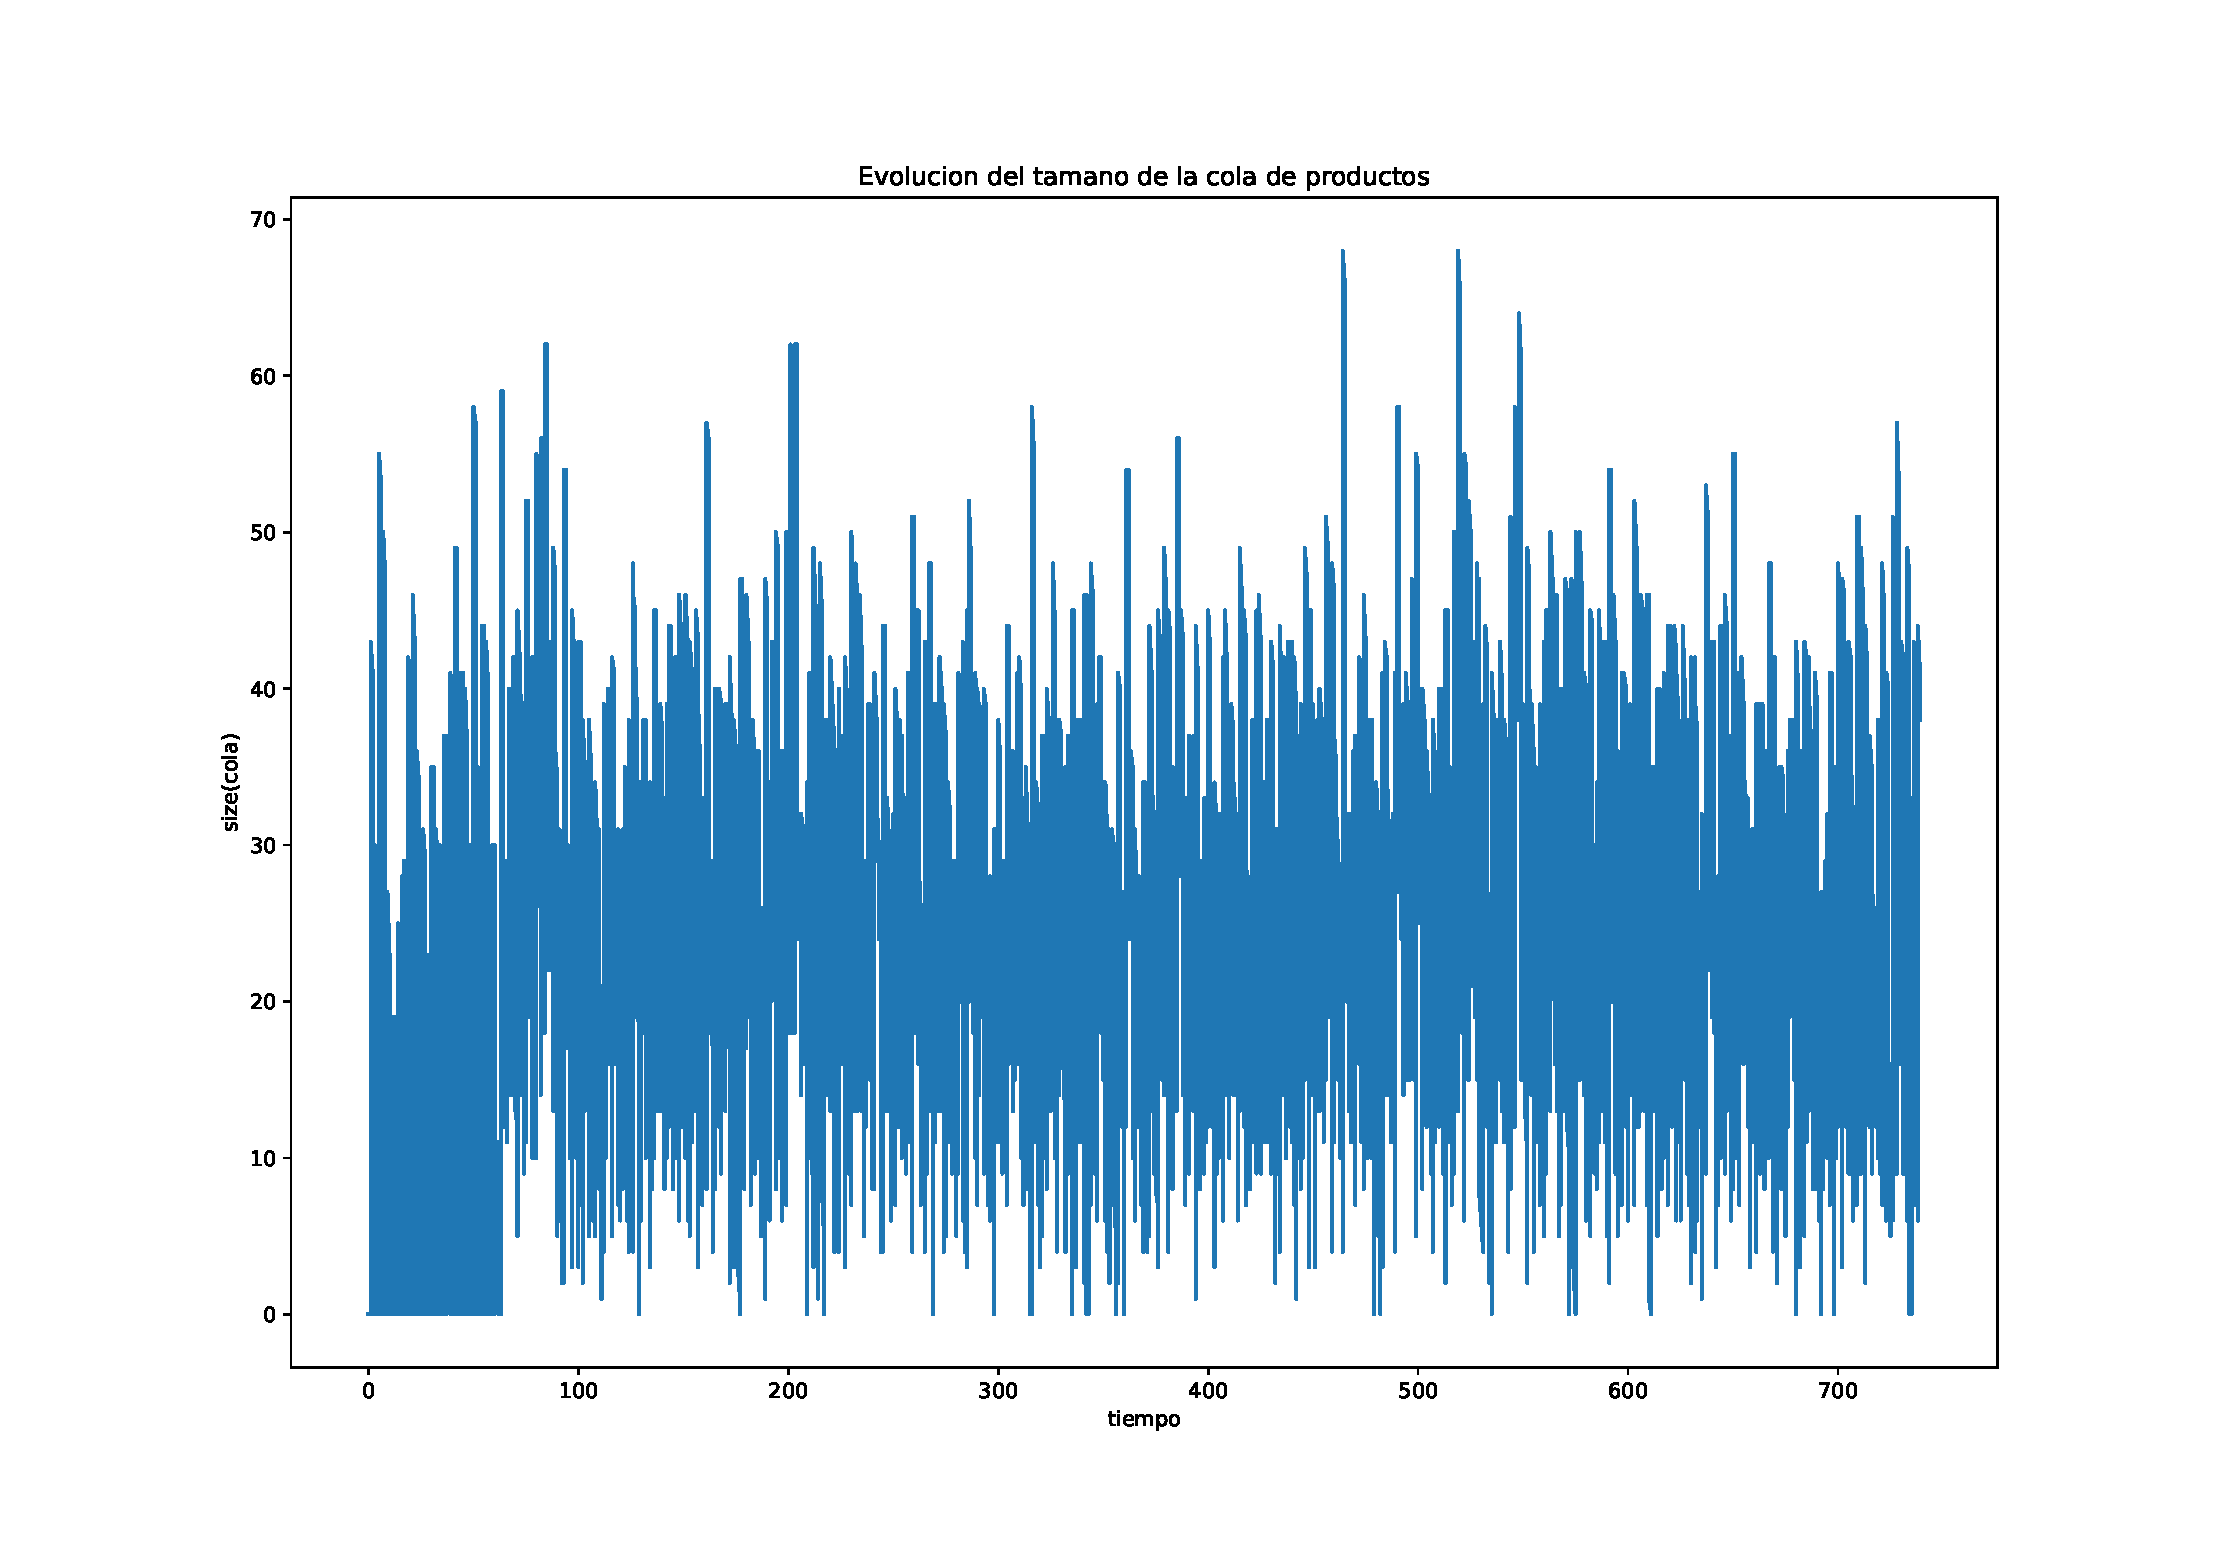
\includegraphics[width=1\textwidth]{img/EvolucionInventario50} 
	\caption{Evolución del tamaño del inventario para $n=50$.} 
	\label{fig:EvolucionInventario50} 
\end{figure}

\begin{figure}[h] 
	\centering 
	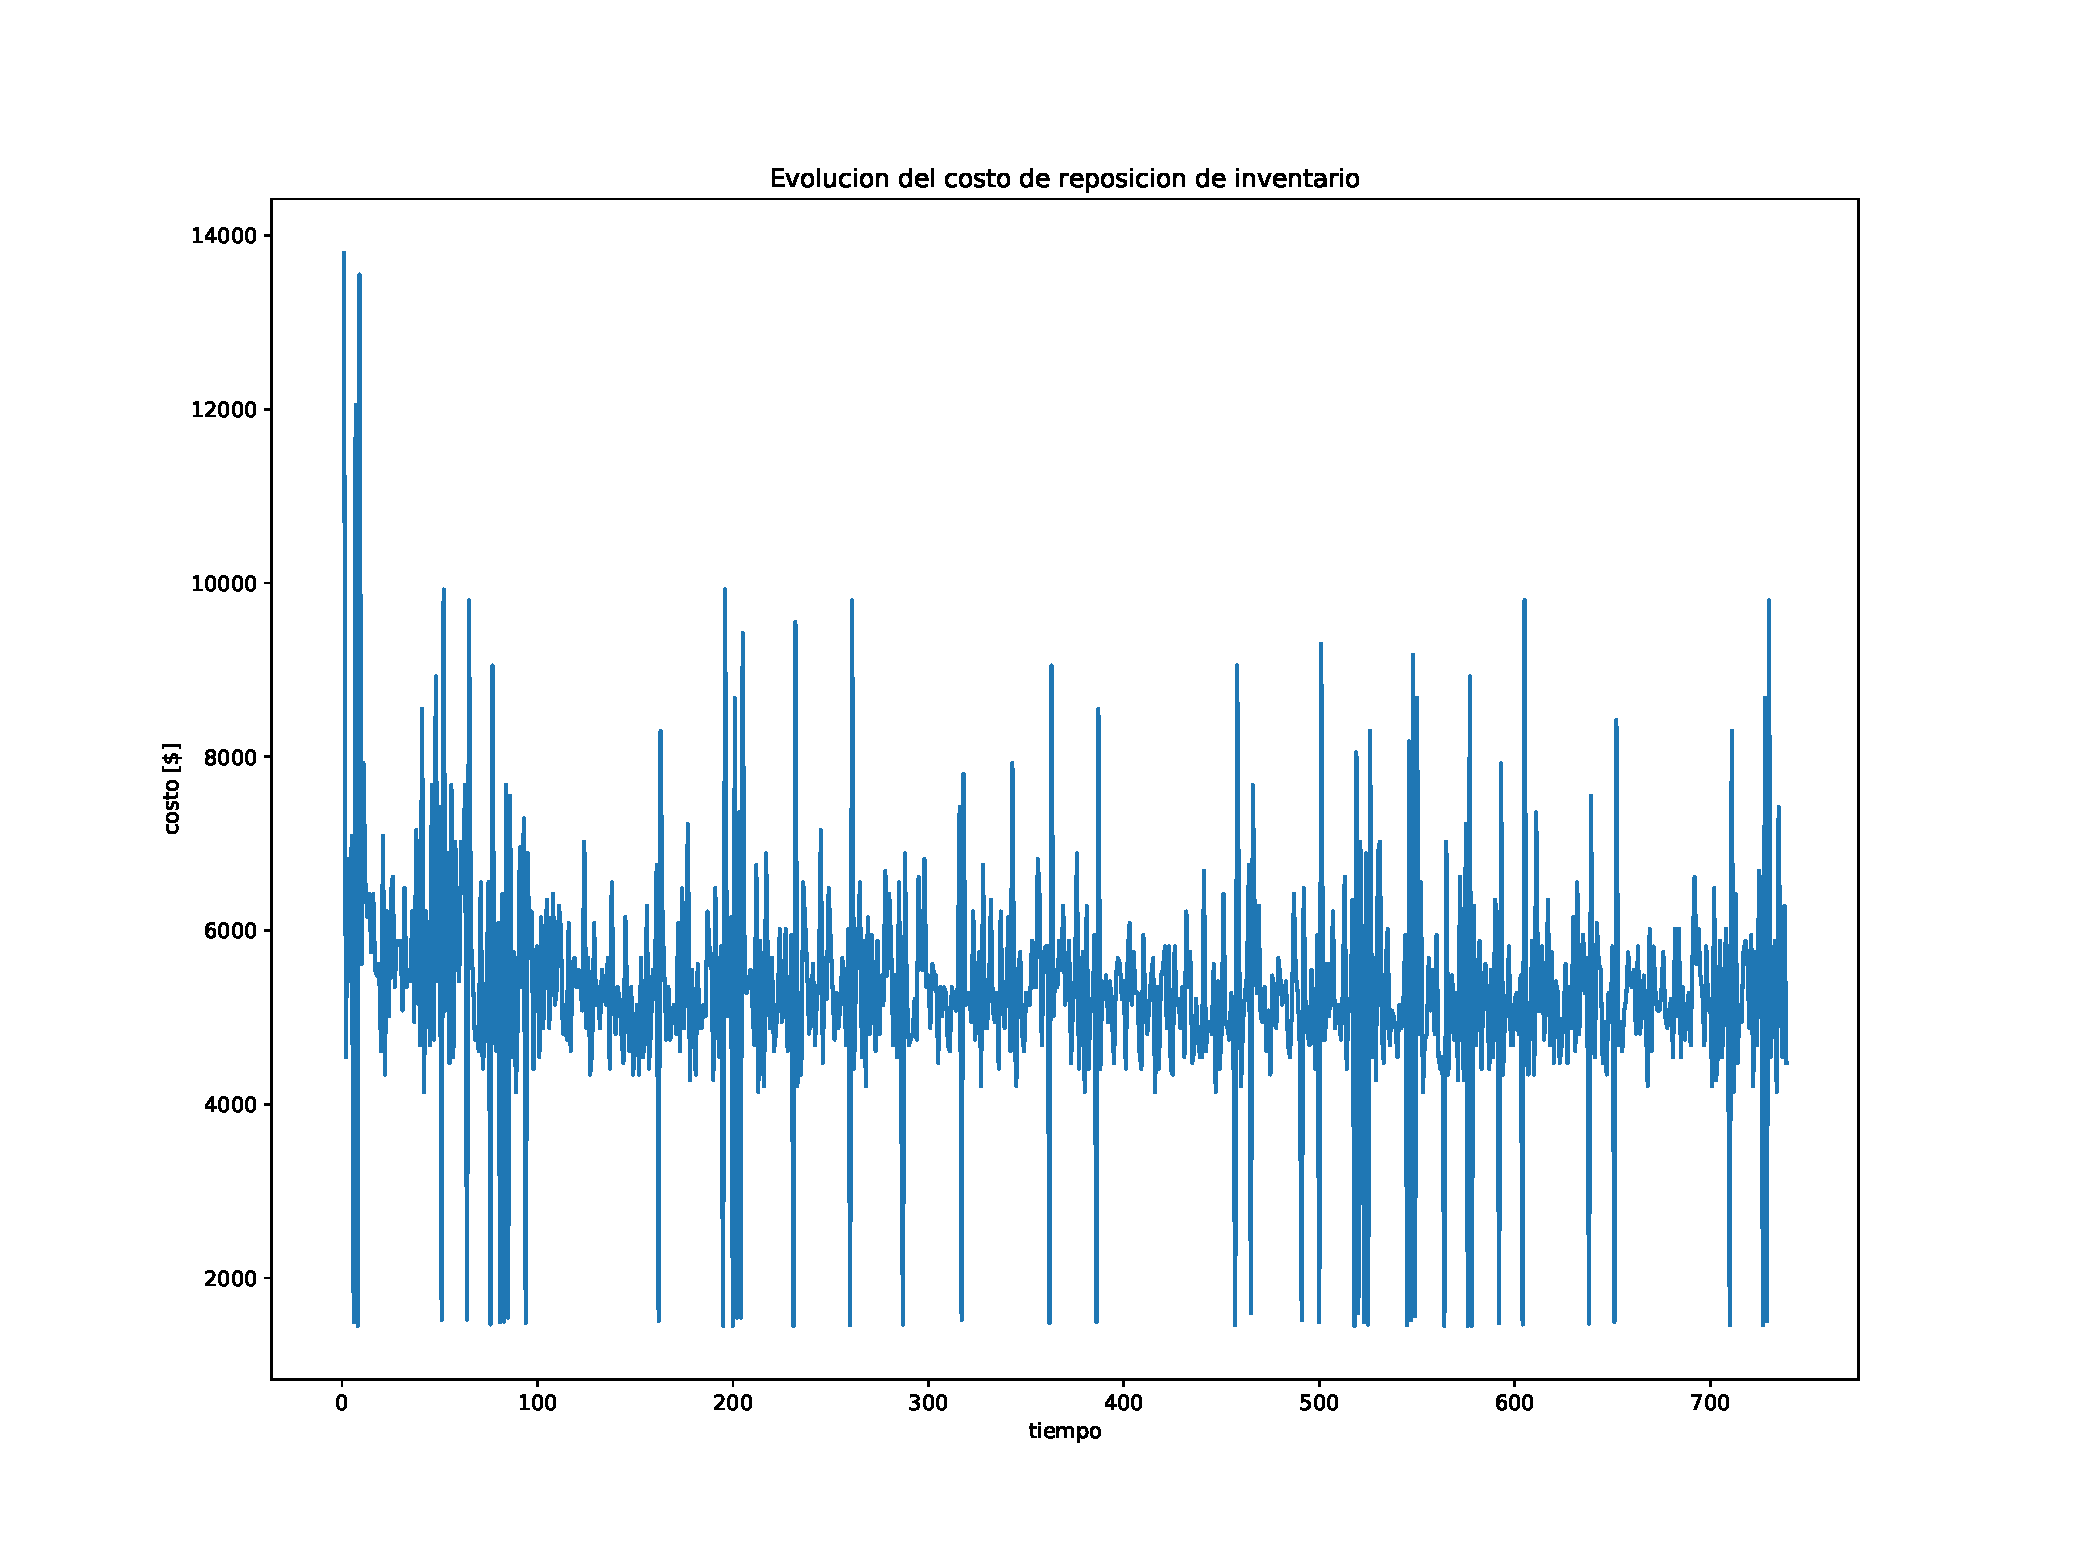
\includegraphics[width=1\textwidth]{img/CostoReposicion50} 
	\caption{Evolución del costo por reposición de inventario para $n=50$.} 
	\label{fig:CostoReposicion50} 
\end{figure}

\begin{figure}[h] 
	\centering 
	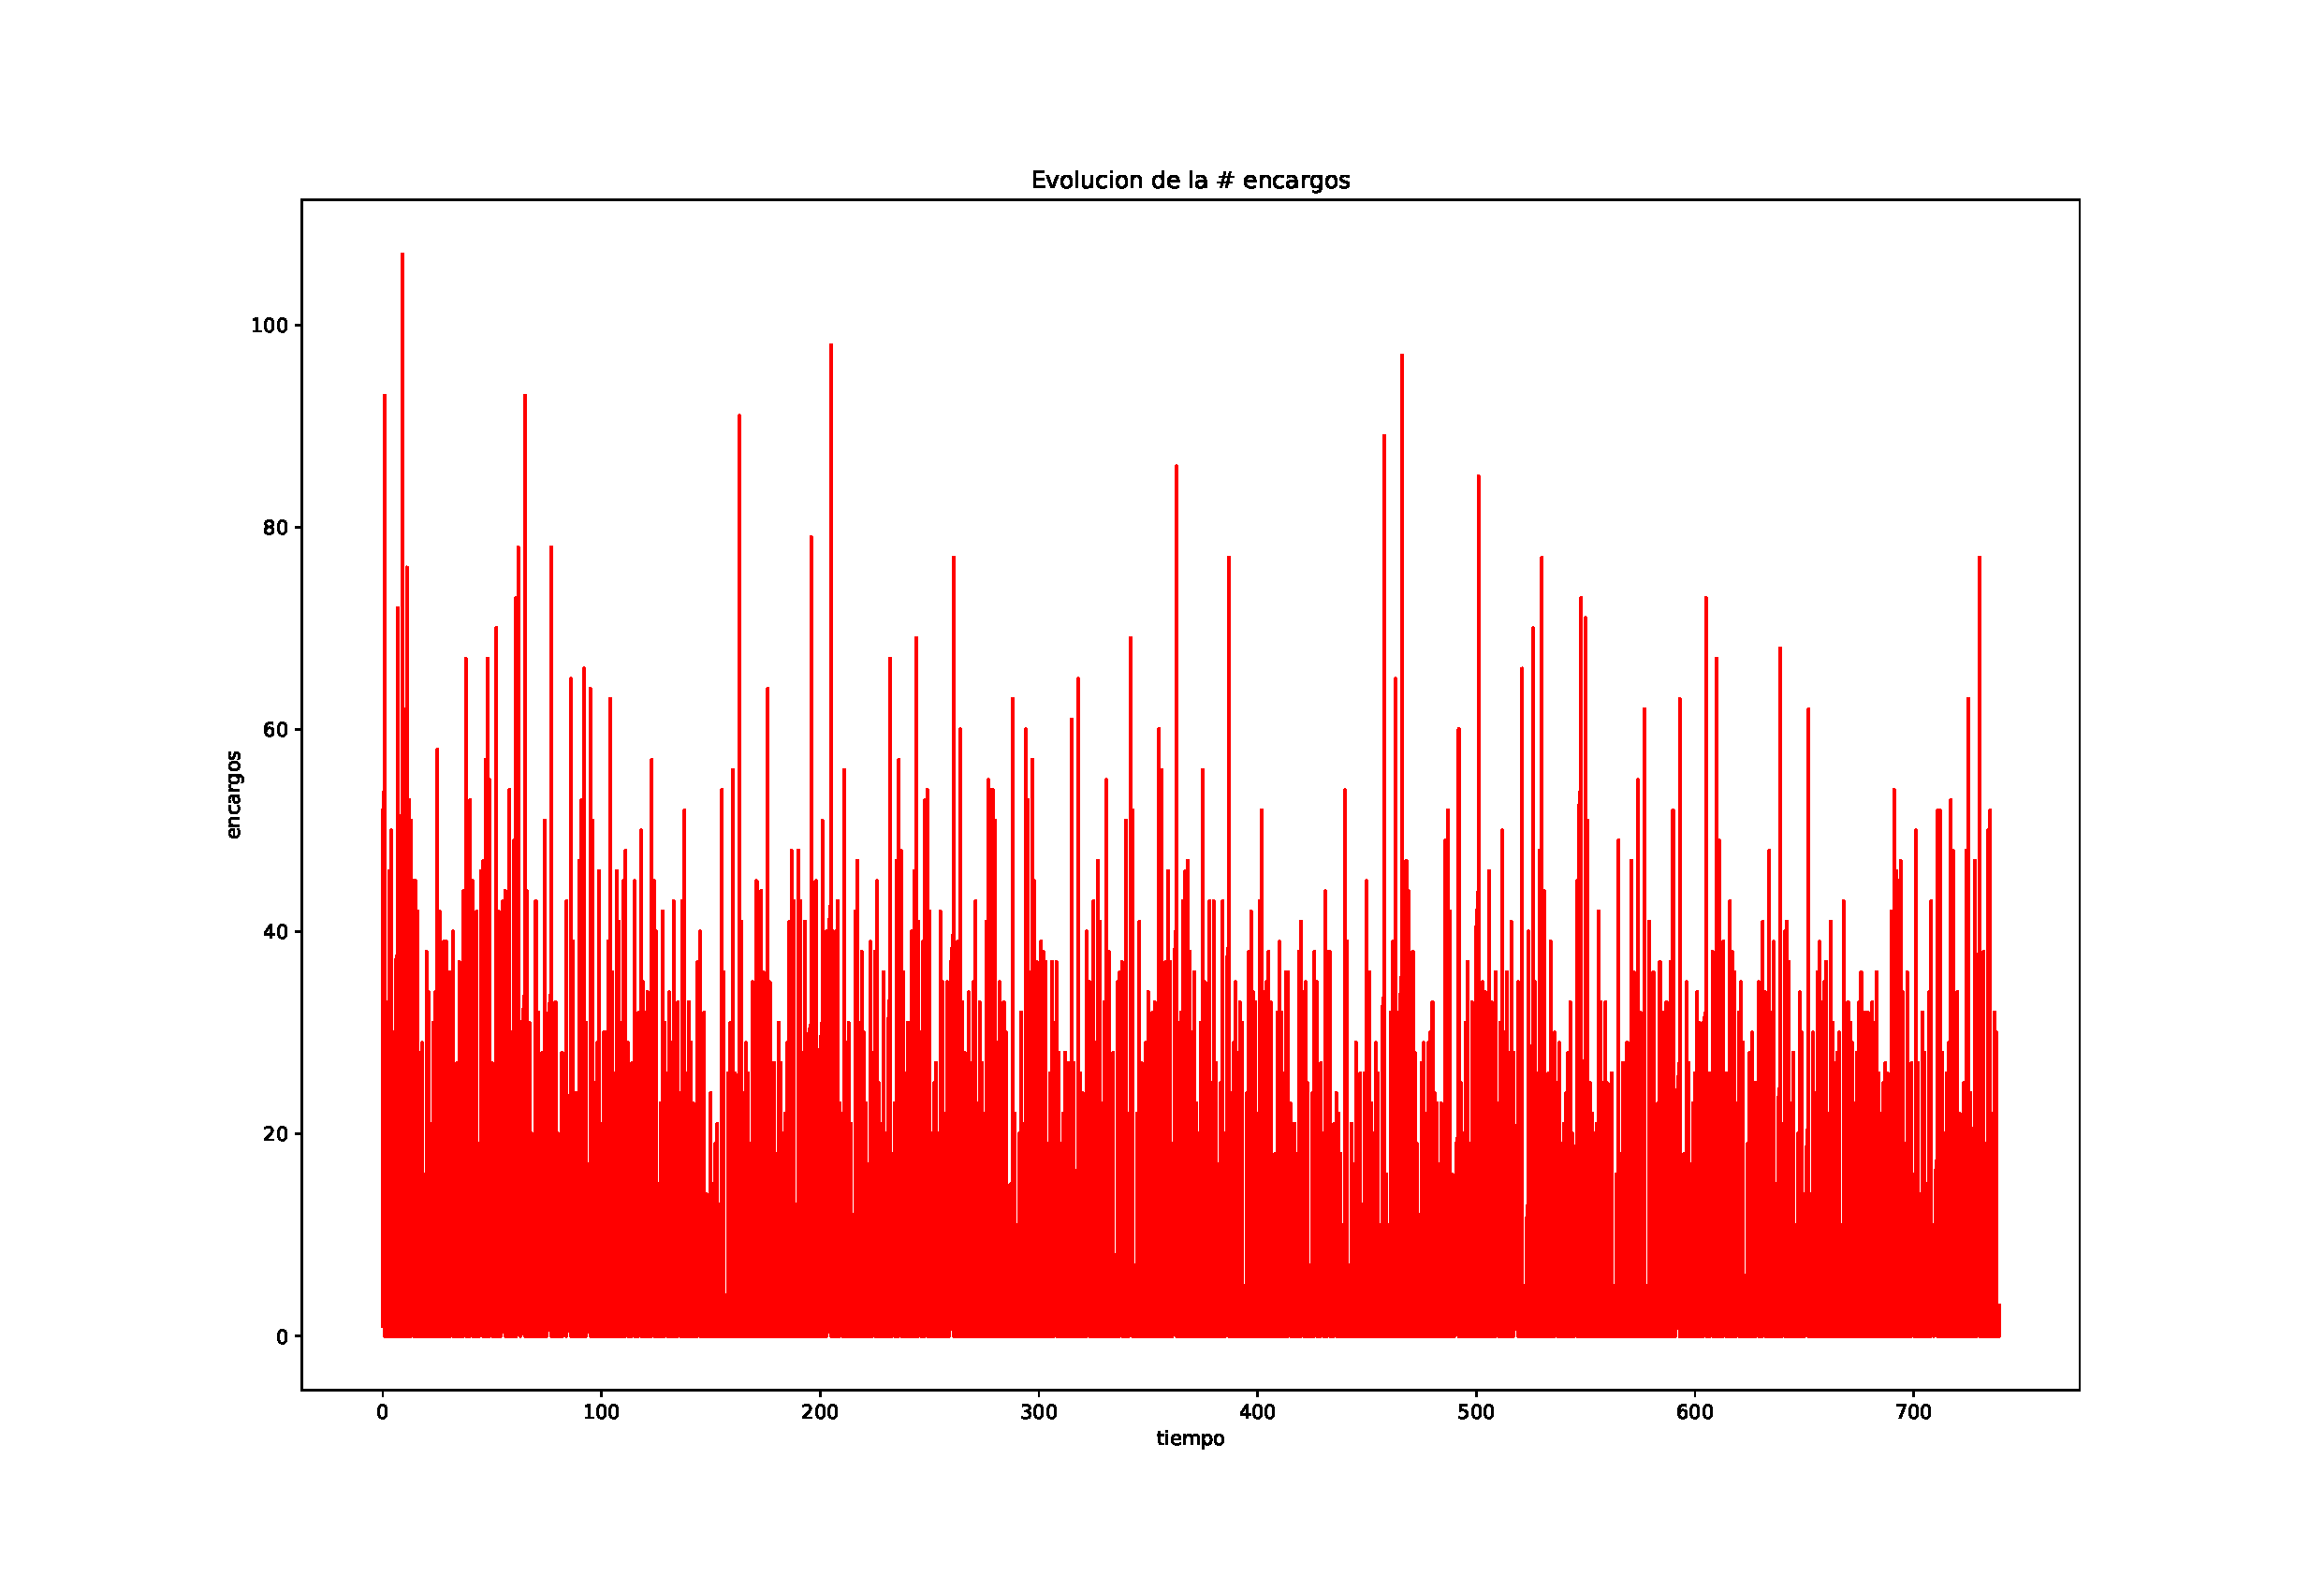
\includegraphics[width=1\textwidth]{img/EvolucionEncargos50} 
	\caption{Evolución de la cantidad de encargos para $n=50$.} 
	\label{fig:EvolucionEncargos50} 
\end{figure}
\FloatBarrier

Como siguiente análisis se procedió a disminuir la política de reposición a $n=10$, con el objeto de evaluar la evolución de los parámetros anteriores. A diferencia del caso anterior se realizarán encargos de materia prima a los proveedores sólo en caso que el nivel del inventario sea menor a $10$. Se espera que el costo baje si el inventario estaba sobredimensionado para la política de reposición anterior o que se produzca una menor cantidad de encargos si por el contrario estaba subdimensionado.

\begin{figure}[h]
	\centering 
	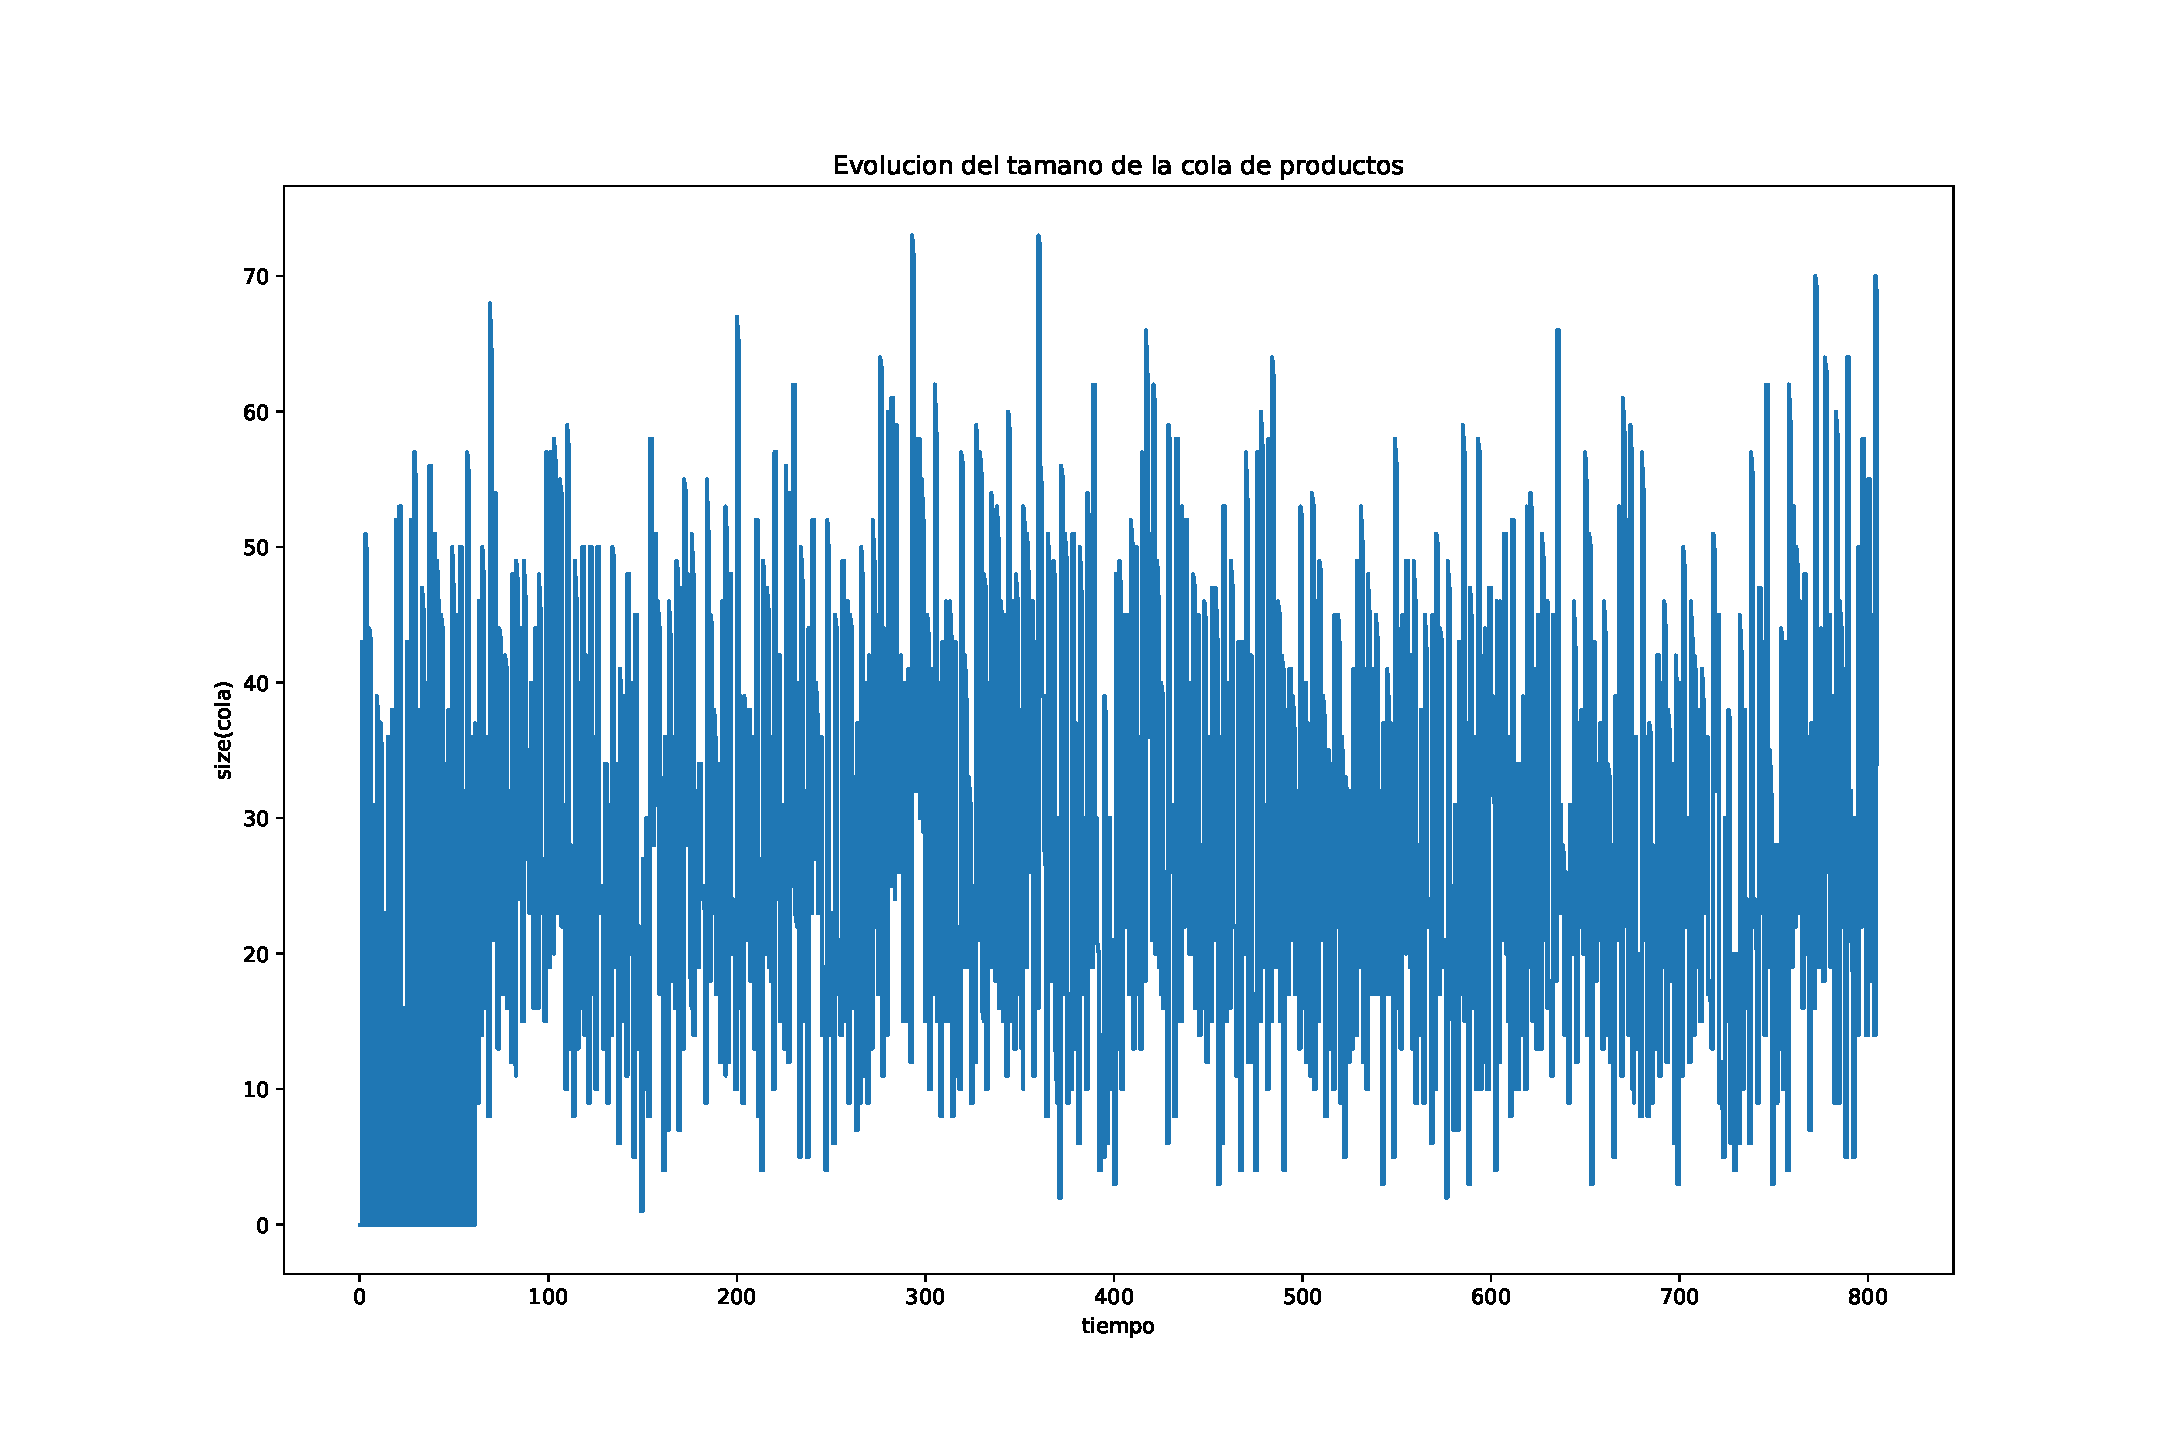
\includegraphics[width=1\textwidth]{img/EvolucionInventario10} 
	\caption{Evolución del tamaño del inventario para $n=10$.} 
	\label{fig:EvolucionInventario10} 
\end{figure}

\begin{figure}[h] 
	\centering 
	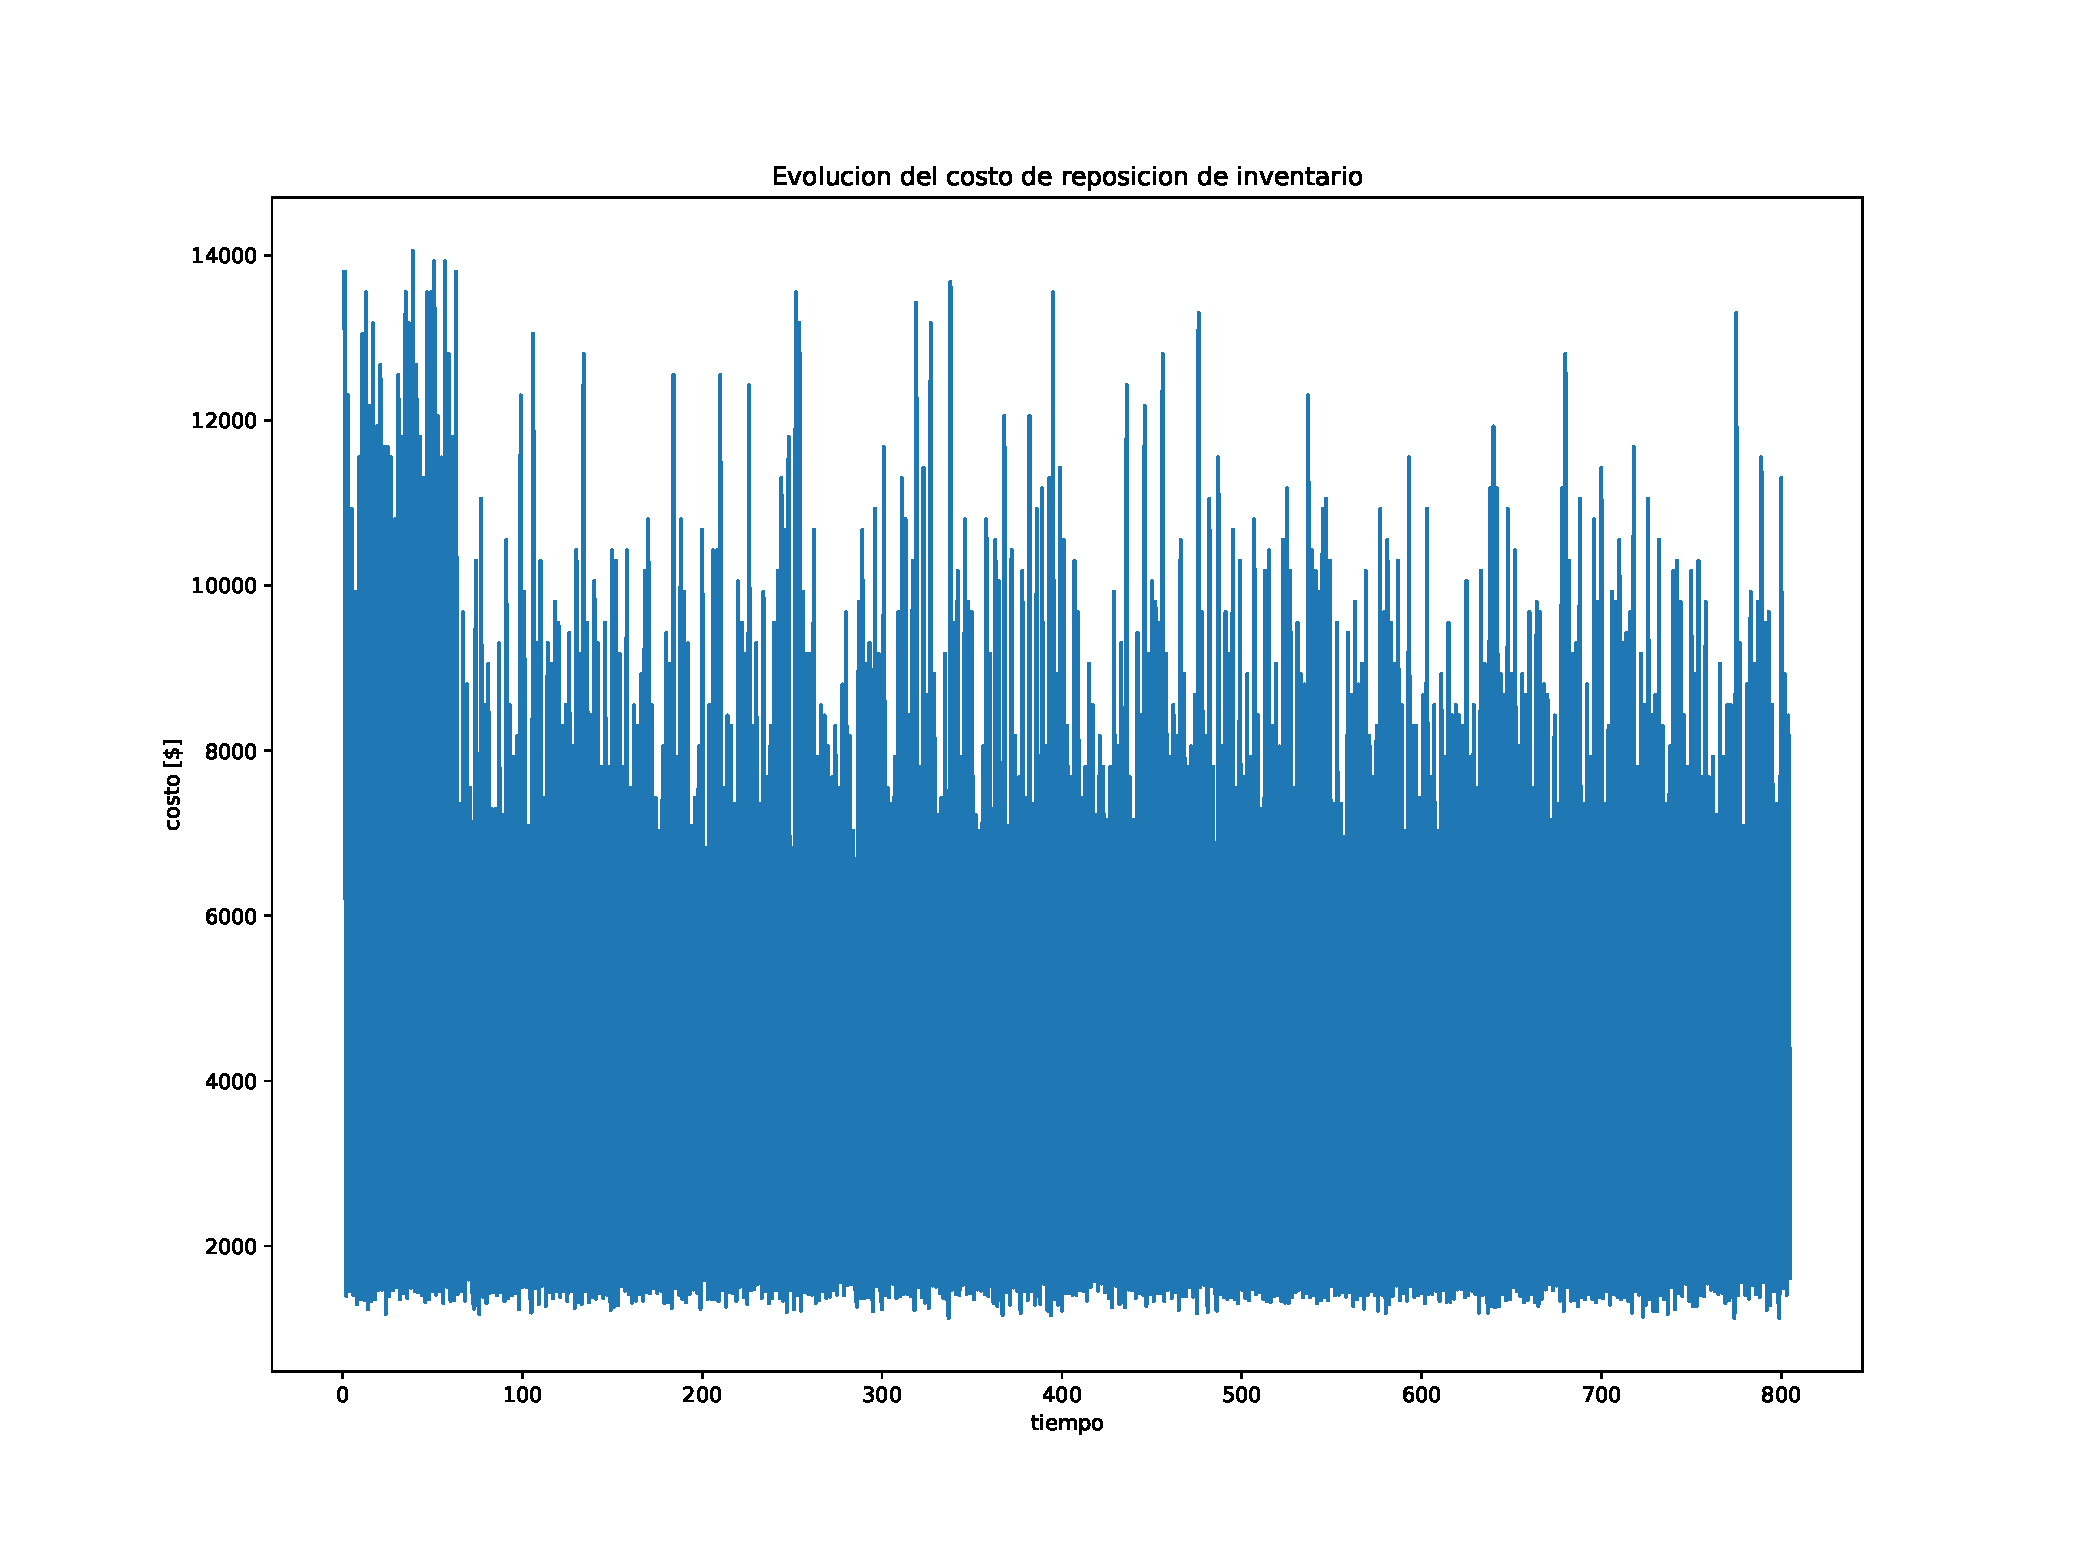
\includegraphics[width=1\textwidth]{img/CostoReposicion10} 
	\caption{Evolución del costo por reposición de inventario para $n=10$.} 
	\label{fig:CostoReposicion10} 
\end{figure}

\begin{figure}[h] 
	\centering 
	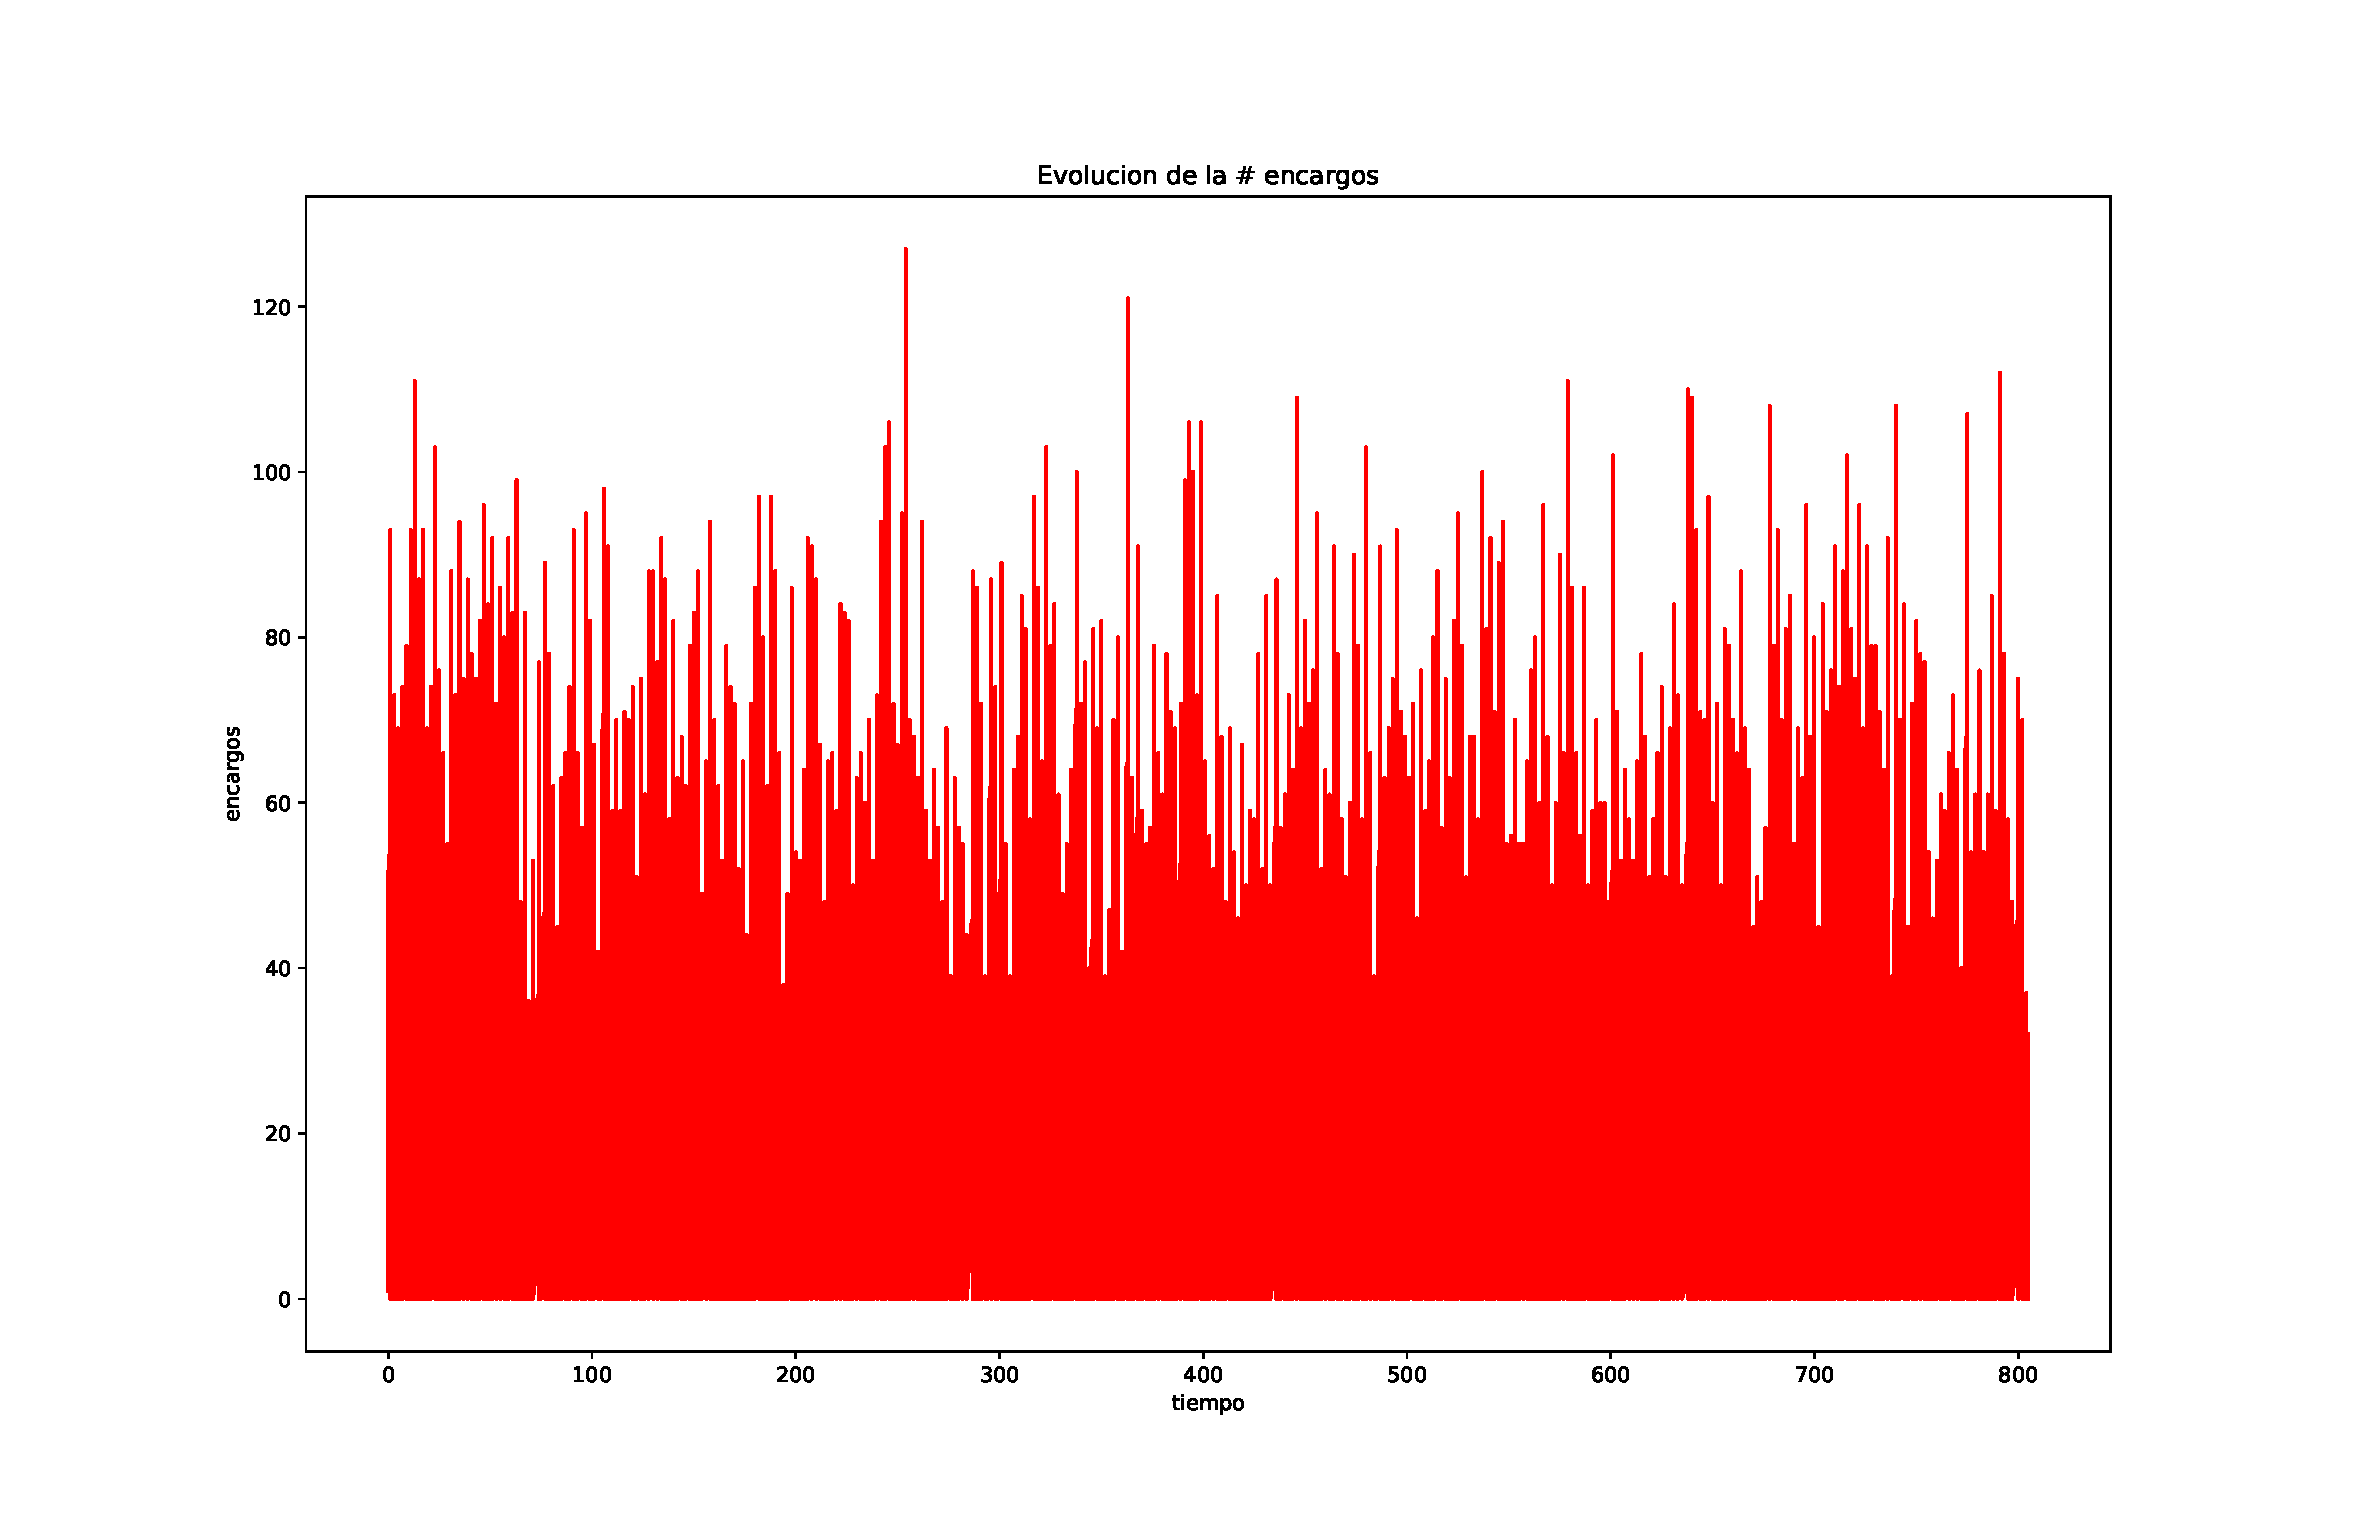
\includegraphics[width=1\textwidth]{img/EvolucionEncargos10} 
	\caption{Evolución de la cantidad de encargos para $n=10$.} 
	\label{fig:EvolucionEncargos10} 
\end{figure}
\FloatBarrier
Se observa que el costo por reposición y mantenimiento de unidades en el inventario se torna mucho más inestable, aumentando levemente en promedio. También se observa un aumento de la cantidad de encargos como así también una mayor variabilidad de la cantidad de productos en el inventario. Estos últimos dos comportamientos justifican el aumento en el costo.
De esto se puede concluir que una política de reposición con un parámetro $n$ tan bajo no resulta eficiente.

Para la elaboración de una unidad de producto es necesario que haya disponibles una unidad de cada insumo. Cada uno de los insumos de los que se compone el producto es provisto por un tipo de proveedor distinto, i.e. el insumo A es provisto por un proveedor inmediato, el insumo B por un proveedor por múltiplo de cantidad fija y el insumo C por un proveedor por encargo que entrega al mes siguiente de efectuado el pedido. En las simulaciones se pudo observar que cada vez que arriba el insumo C se consume al instante en la elaboración de productos pues los insumos A y B ya estaban previamente disponibles para ellos. Por este motivo, en todo momento la cola C de la Figura~\ref{fig:esquema-del-problema} tiene largo $0$. También se puede notar que debido a la política de entrega del proveedor por múltiplo de cantidad fija, en la cola del insumo B siempre quedan remanentes de los pedidos anteriores y por lo tanto el tamaño de esta cola crece sostenidamente.
%%%%%%%%%%%%%%%%
% Figuras aquí %
%%%%%%%%%%%%%%%%
\subsubsection{Conclusiones}
Se comprobó la utilidad del formalismo DEVS y en particular de la herramienta CD++ para el modelado y simulación de sistemas con dinámicas por eventos. Al producirse eventos de manera aleatoria no es posible modelizarlos utilizando simuladores basados en una base de tiempo discreta, pues la ocurrencia de un evento de entrada es impredecible y por lo tanto el paso de simulación debería ser lo suficientemente pequeño como para coincidir con los eventos. En caso de adaptar el paso de simulación a la aparición de eventos hace que el tiempo necesario para realizar una simulación crezca exponencialmente.

Se simuló el comportamiento de un sistema de inventario de una industria considerando clientes de distinto tipo y proveedores con distintos comportamientos. Los insumos entregados por los proveedores se utilizan para elaborar el único producto de esta industria. Cada insumo y cada producto se representa a partir de su fecha de vencimiento. Los instantes en los que los clientes realizan pedidos, como la cantidad de unidades que piden y las fechas de vencimiento de los insumos y los productos responden a variables aleatorias con determinadas distribuciones de probabilidad.y cuyos. En particular, para este trabajo se consideraron tasas de arribo de pedidos de clientes que siguen una distribuciones exponenciales.

Se descompuso al problema en tres niveles jerárquicos: a) un nivel superior o \textit{top model} donde se encuentran la industria, los clientes y los proveedores, b) un segundo nivel dentro de la industria compuesto por el inventario, el control de inventario y la atención del cliente, y c) un tercer nivel de atención al cliente conformado por la atención al cliente y el control de calidad.

Para validar el comportamiento del sistema, en la sección~\ref{sec:PP} se verificó de forma independiente el comportamiento de cada bloque excitándolos con entradas conocidas y analizando si los resultados obtenidos correspondían con los esperados.

Durante el desarrollo del trabajo nos encontramos con un problema de simultaneidad de eventos. Por un lado, el control de inventario realiza un pedido a sus proveedores a principio de cada mes. Por el otro lado, el proveedor por encargo entrega en ese mismo momento los insumos que le fueron encargados al inicio del mes. Esta simultaneidad fue \textit{evitada} haciendo que el proveedor entregue cada $0.999~\textrm{mes}$. 

Por último, a lo largo del desarrollo de las simulaciones con la herramienta CD++ se encotraron algunos inconvenientes: a) la variable \texttt{nextChange()} no representa el tiempo entre la última transición interna y la próxima sino el tiempo que falta hasta dicha transición, b) el archivo \texttt{.ma} no distingue parámetros en mayúsculas y minúsculas (no es \textit{case-sensitive}) y c) el archivo de salida de la simulación no guarda toda la información de los mensajes intercambiados por los bloques a lo largo de la simulación. Por este último motivo, en las funciones de salida de los atómicos se agregaron mensajes propios que utilizamos para analizar el comportamiento de la simulación y filtrar información que luego procesamos con un script de python. Para este trabajo práctico se utilizó el simulador CD++ en su versión \textit{standalone} por consola.











\appendix
\section{Código Implementado}

\url{https://github.com/TwinT/DEVS-Inventario}

% Please don't exchange the bibliographystyle style
\bibliographystyle{IEEEtran.bst}
% AUTHOR: Include your bib file here
\bibliography{IEEEexample}

\end{document}

